\chapter{Metodologia}

Este capítulo apresenta os procedimentos metodológicos adotados para o desenvolvimento, implementação e avaliação do sistema fotovoltaico automatizado proposto neste trabalho. A pesquisa possui abordagem quantitativa, sendo conduzida por meio do desenvolvimento de um protótipo experimental e da comparação entre resultados obtidos por simulação computacional e dados experimentais coletados em condições reais de operação.

metodologia foi estruturada de forma a contemplar todas as etapas necessárias para o desenvolvimento e a validação do sistema proposto. A metodologia foi estruturada em quatro etapas principais: seleção dos materiais e construção do protótipo experimental; desenvolvimento da lógica de funcionamento do sistema; modelagem computacional no ambiente MATLAB/Simulink; e realização dos ensaios experimentais para validação do modelo computacional.

Após a implementação do protótipo, foram realizados ensaios experimentais em ambiente externo, sob condições reais de operação, utilizando simultaneamente um sistema automatizado e um sistema com painel fixo como referência. Durante os experimentos, foram registradas as variáveis elétricas necessárias para a avaliação do desempenho dos dois sistemas. Os dados experimentais obtidos durante os ensaios foram organizados, processados e comparados aos resultados gerados pelo modelo computacional desenvolvido no MATLAB/Simulink. 

Essa comparação permitiu avaliar a capacidade do modelo em representar o comportamento observado no protótipo físico, validando sua utilização como ferramenta de apoio para a análise do desempenho do sistema fotovoltaico automatizado. A Figura~\ref{fig:fluxo_metodologia} apresenta, de forma resumida, as principais etapas que compõem a metodologia adotada neste trabalho.

\begin{figure}[H]
    \centering
    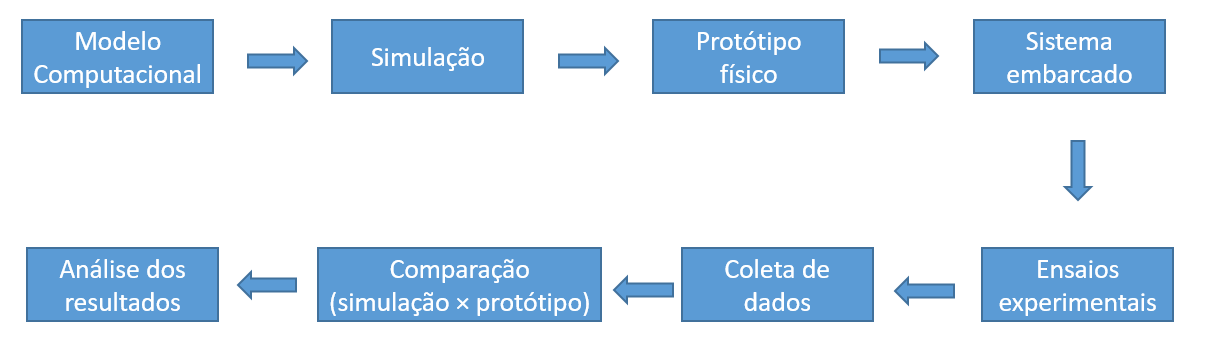
\includegraphics[width=0.95\textwidth]{Figuras/fluxo_metodologia}
    \caption{Fluxograma das etapas metodológicas desenvolvidas neste trabalho.}
    \label{fig:fluxo_metodologia}
    \fonte{Elaborado pelo autor.}
\end{figure}

As seções seguintes descrevem detalhadamente os materiais empregados, a arquitetura de hardware e software do sistema, o desenvolvimento do modelo computacional, os procedimentos experimentais adotados e os métodos utilizados para análise e comparação dos resultados.

\section{Materiais e Hardware}

    \subsection{Painel Fotovoltaico}

O protótipo experimental foi desenvolvido utilizando um módulo fotovoltaico policristalino com potência nominal de 3~W, tensão nominal de 6~V em corrente contínua e dimensões aproximadas de 21~cm $\times$ 13~cm, conforme apresentado na Figura~\ref{fig:placa_solar}. A escolha desse módulo deve-se à sua compatibilidade com a proposta experimental, permitindo a realização de ensaios comparativos entre um sistema automatizado e um sistema de painel fixo com baixo custo de implementação.

\begin{figure}[H]
    \centering
    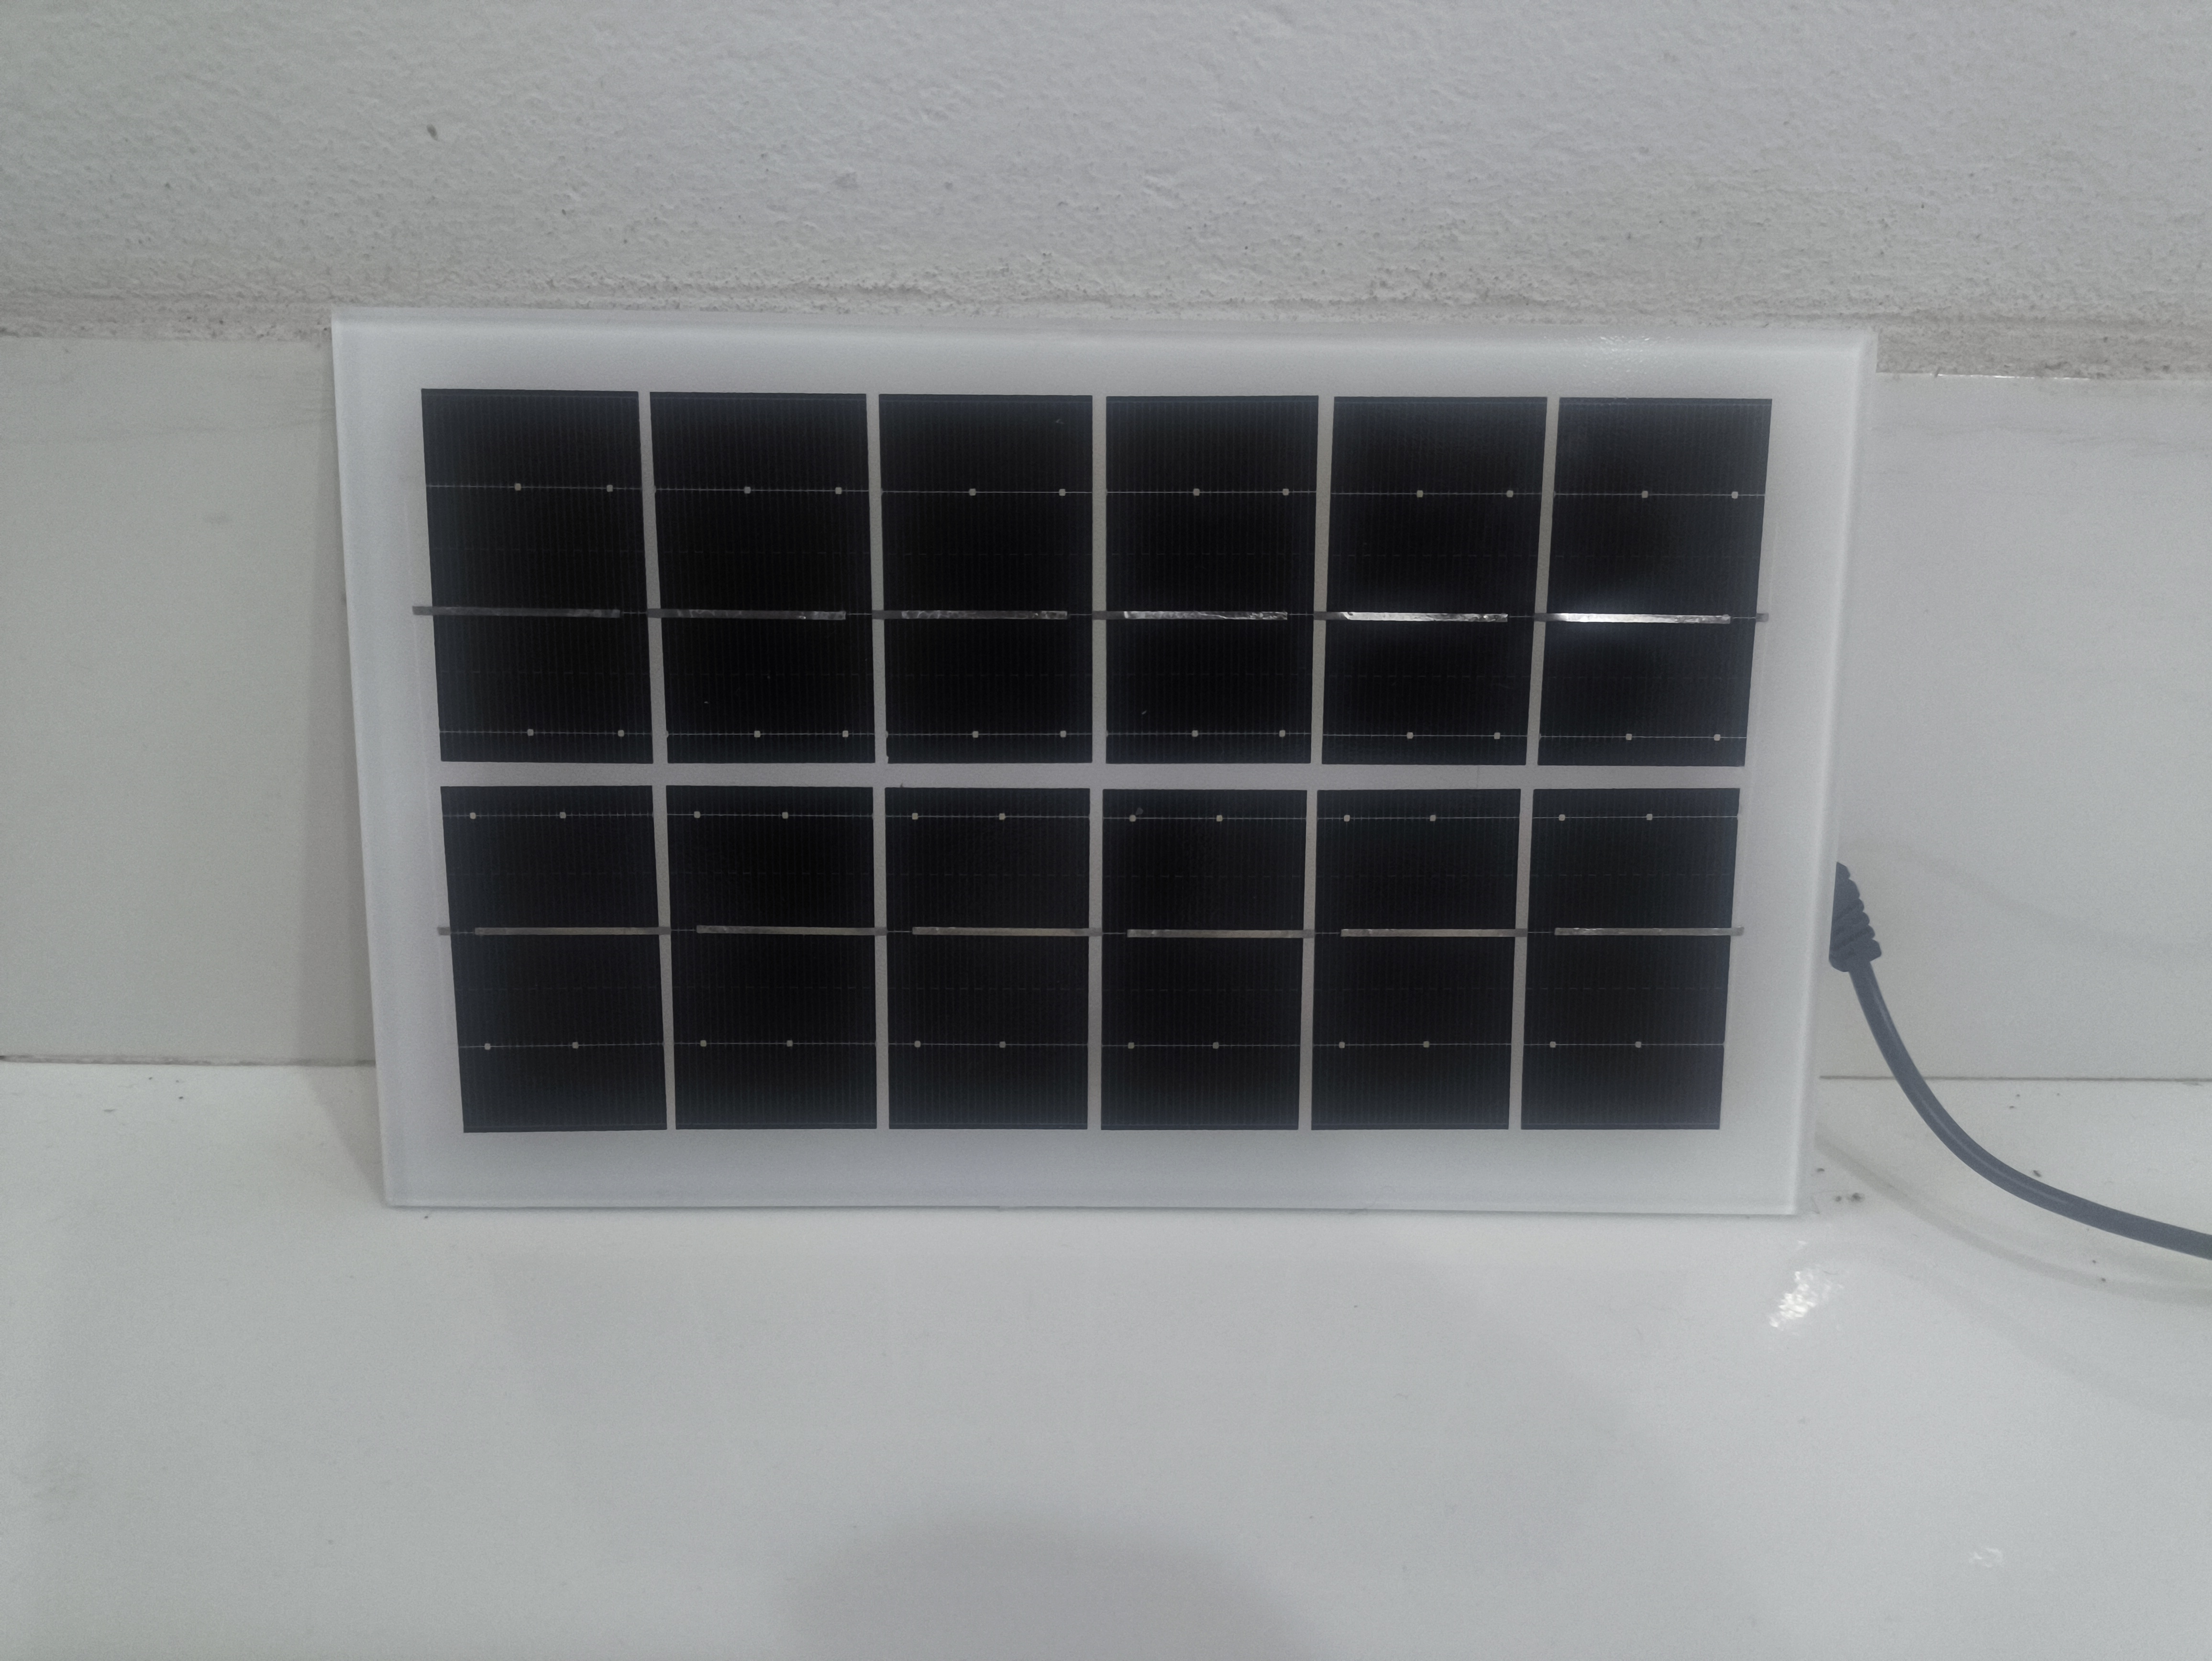
\includegraphics[width=0.7\textwidth]{Figuras/placa_solar.jpg}
    \caption{Painel fotovoltaico utilizado no protótipo experimental.}
    \label{fig:placa_solar}
    \fonte{Autor (2026).}
\end{figure}

O painel fotovoltaico constituiu o elemento responsável pela conversão da radiação solar em energia elétrica e pela geração das variáveis elétricas monitoradas durante os experimentos. As medições de tensão e corrente obtidas por meio dos sensores instalados no sistema foram utilizadas para o cálculo da potência elétrica instantânea e para a comparação do desempenho entre o sistema automatizado e o sistema com painel fixo.

Embora apresente potência reduzida quando comparado aos módulos empregados em instalações comerciais, o painel utilizado possui características suficientes para aplicações experimentais, permitindo reproduzir o comportamento de sistemas fotovoltaicos de maior porte em escala reduzida. Essa abordagem é frequentemente adotada em pesquisas experimentais por possibilitar a avaliação de estratégias de controle e posicionamento com menor custo e maior facilidade de implementação.

Para possibilitar uma comparação direta entre as duas configurações avaliadas, foram utilizados dois painéis fotovoltaicos com as mesmas especificações durante os experimentos. Um permaneceu em posição fixa, enquanto o outro foi acoplado ao mecanismo automatizado de movimentação, possibilitando a comparação direta entre as duas configurações sob as mesmas condições ambientais.

As especificações técnicas dos módulos foram fornecidas pelo fabricante considerando as Condições Padrão de Teste (\textit{Standard Test Conditions} -- STC), conforme estabelecido pela norma IEC 61215. Nessas condições, os painéis operam próximos de sua potência nominal \cite{iec2016}.

Durante os experimentos, os módulos foram instalados em ambiente externo e submetidos às condições reais de operação, nas quais a irradiância solar e a temperatura das células variam continuamente ao longo do dia. Dessa forma, os valores obtidos representam o comportamento dos sistemas em condições reais de funcionamento, permitindo avaliar a influência do posicionamento automatizado sobre a geração de energia elétrica.

\subsection{Microcontrolador Arduino}

A unidade de processamento do protótipo foi implementada utilizando a plataforma Arduino Uno, baseada no microcontrolador ATmega328P. A placa opera a 16 MHz, possui 14 portas digitais de entrada e saída, das quais seis podem operar como saídas PWM (\textit{Pulse Width Modulation}), além de seis entradas analógicas destinadas à aquisição de sinais provenientes de sensores \cite{arduino2023}. A placa utilizada é apresentada na Figura~\ref{fig:arduino_uno}. 
\begin{figure}[H]
    \centering
    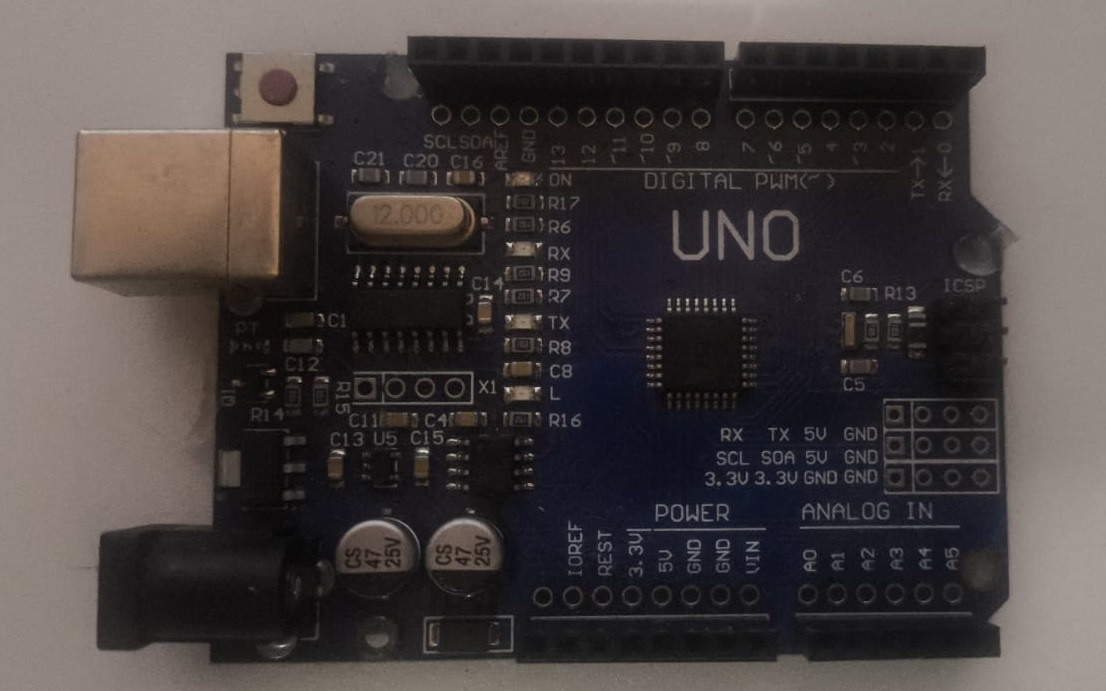
\includegraphics[width=0.6\textwidth]{Figuras/Placa Arduino Uno.jpeg}
    \caption{Placa Arduino Uno utilizada no protótipo.}
    \label{fig:arduino_uno}
    \fonte{Autor (2026).}
\end{figure}

A escolha dessa plataforma foi motivada por sua capacidade de atender aos requisitos computacionais do sistema desenvolvido, que envolvem aquisição de dados, processamento em tempo real, controle de atuadores e comunicação com dispositivos periféricos. Além disso, a disponibilidade de interfaces digitais, entradas analógicas e bibliotecas específicas simplifica a integração com sensores, servomotores, módulos RTC, display LCD e dispositivos de armazenamento em cartão SD.

No protótipo desenvolvido, o Arduino Uno atuou como unidade central de controle, executando continuamente o algoritmo responsável pelo monitoramento e pelo posicionamento automatizado do painel fotovoltaico. Durante a operação do sistema, o microcontrolador realiza a leitura dos sensores de tensão e corrente, calcula a potência elétrica instantânea a partir dessas medições, determina o ângulo de posicionamento do painel com base no horário fornecido pelo módulo RTC, aciona o servomotor por meio de sinais PWM, atualiza as informações exibidas no display LCD e registra automaticamente os dados experimentais no cartão microSD para posterior análise.

Dessa forma, o Arduino Uno atuou como elemento central do sistema embarcado, coordenando todas as etapas de monitoramento, controle e registro das informações experimentais. A lógica de funcionamento implementada no microcontrolador é apresentada na Seção~3.2.

\subsection{Servomotor}

O acionamento mecânico do painel fotovoltaico foi realizado por meio de um servomotor modelo MG996R, apresentado na Figura~\ref{fig:servo_mg996r}. A escolha desse dispositivo deve-se ao seu elevado torque, à boa precisão de posicionamento angular e à facilidade de integração com a plataforma Arduino, características adequadas para aplicações de controle de posição em sistemas automatizados.

\begin{figure}[H]
    \centering
    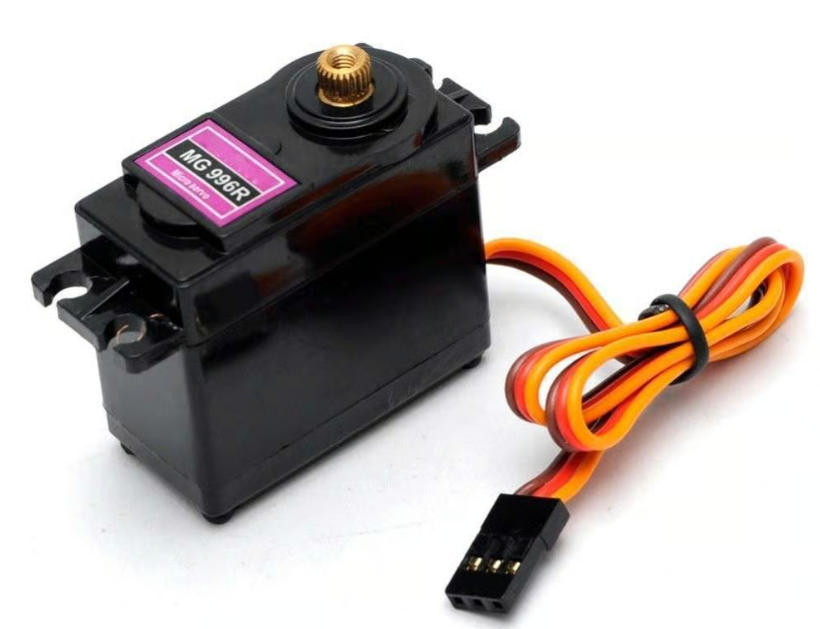
\includegraphics[width=0.6\textwidth]{Figuras/servo motor.png}
    \caption{Servomotor MG996R utilizado no protótipo.}
    \label{fig:servo_mg996r}
    \fonte{Adaptado de Eletrônica Castro (2026).}
\end{figure}

O servomotor MG996R possui faixa de operação aproximada de 0° a 180° e realiza o posicionamento angular a partir de sinais PWM (\textit{Pulse Width Modulation}) enviados pelo microcontrolador. Essa característica proporciona boa precisão e repetibilidade dos movimentos, tornando o dispositivo adequado para aplicações de controle de posição em sistemas automatizados \cite{towerpro2019,arduino_servo}.

No sistema desenvolvido, o servomotor foi responsável pelo posicionamento automático do painel fotovoltaico ao longo do período de operação. O ângulo de rotação foi determinado pelo algoritmo implementado no Arduino com base no horário fornecido pelo módulo RTC, realizando o deslocamento gradual do painel entre as posições correspondentes ao nascer e ao pôr do Sol.

Considerando que o posicionamento do painel influencia diretamente a incidência da radiação solar sobre sua superfície, A utilização do servomotor possibilitou implementar o controle automático da posição angular do painel fotovoltaico sem a necessidade de mecanismos adicionais de posicionamento, contribuindo para simplificar a construção do protótipo e reduzir sua complexidade mecânica e eletrônica.


\subsection{Sensores de Corrente e Tensão}

A aquisição das variáveis elétricas do sistema foi realizada por meio de um sensor de corrente ACS712 e de um módulo sensor de tensão baseado em divisor resistivo, apresentados na Figura~\ref{fig:sensores}. Esses dispositivos foram utilizados para monitorar continuamente a corrente e a tensão produzidas pelo painel fotovoltaico durante os ensaios experimentais, fornecendo as informações necessárias para o cálculo da potência elétrica gerada.

\begin{figure}[H]
    \centering

    \begin{minipage}{0.45\linewidth}
        \centering
        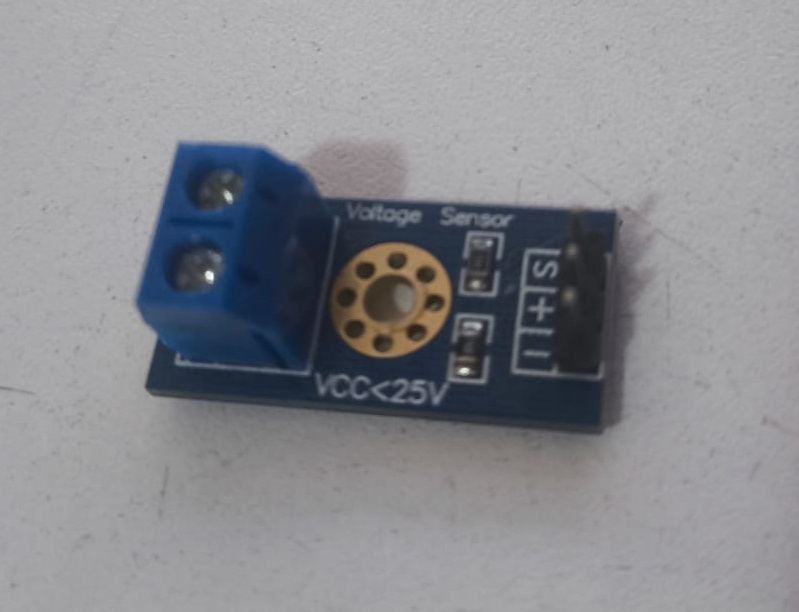
\includegraphics[height=5cm]{Figuras/sensor_tensao.jpeg}

        (a) Sensor de tensão
    \end{minipage}
    \hfill
    \begin{minipage}{0.45\linewidth}
        \centering
        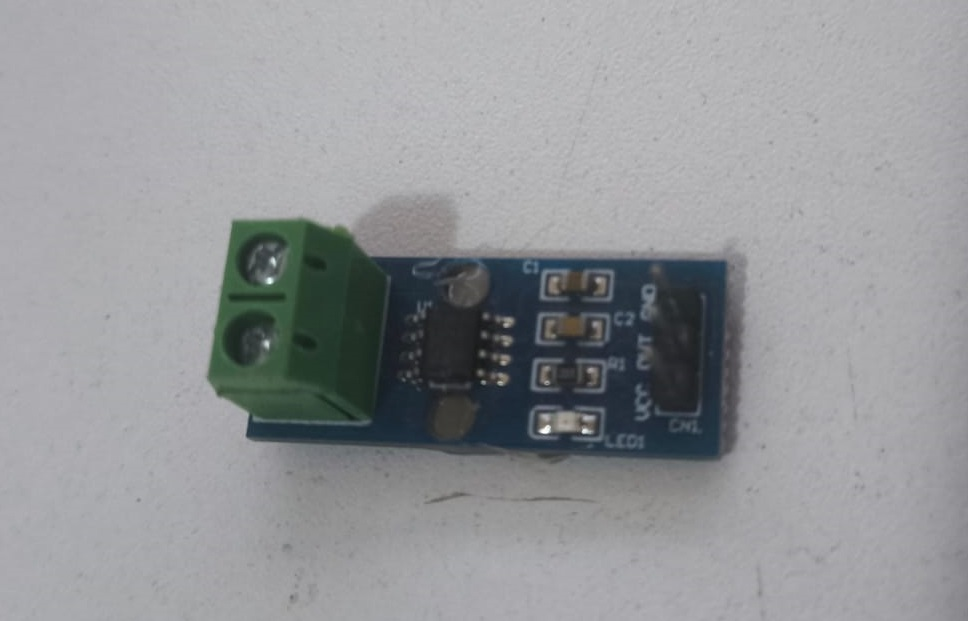
\includegraphics[height=5cm]{Figuras/sensor_corrente.jpeg}

        (b) Sensor de corrente
    \end{minipage}

    \caption{Sensores utilizados para aquisição das grandezas elétricas do sistema.}
    \label{fig:sensores}
    \fonte{Autor (2026).}
\end{figure}

O sensor ACS712, baseado no efeito Hall, realiza a medição indireta da corrente elétrica, disponibilizando ao microcontrolador um sinal analógico proporcional à corrente que circula no circuito, preservando o isolamento elétrico entre o circuito de potência e o circuito de medição \cite{allegro2019,sparkfun_acs712}. O módulo sensor de tensão, por sua vez, utiliza um divisor resistivo para reduzir a tensão aplicada à sua entrada para níveis compatíveis com as entradas analógicas do Arduino, permitindo a medição segura de tensões contínuas de até 25~V \cite{usinainfo2024,sedra2016}.

Os sinais analógicos provenientes dos dois sensores foram adquiridos pelo conversor analógico-digital do Arduino e convertidos em valores de tensão e corrente por meio das rotinas de calibração implementadas no software de controle. A partir dessas grandezas foi calculada, em tempo real, a potência elétrica instantânea produzida pelo painel fotovoltaico, utilizando a Equação~\ref{eq:potencia}.

\begin{equation}
P = V \times I
\label{eq:potencia}
\end{equation}

em que $P$ representa a potência elétrica (W), $V$ corresponde à tensão elétrica (V) e $I$ representa a corrente elétrica (A).

As medições foram realizadas automaticamente em intervalos de um minuto durante todo o período experimental, compreendido entre 06h00 e 18h00. Esse intervalo de aquisição foi adotado para permitir o acompanhamento da variação das grandezas elétricas ao longo do dia e o cálculo da energia acumulada produzida pelos sistemas.

As variáveis elétricas calculadas foram utilizadas para o monitoramento do desempenho do sistema, sendo apresentadas em tempo real no display LCD e registradas automaticamente no cartão microSD, juntamente com a data, o horário e o ângulo de posicionamento do painel fotovoltaico. Posteriormente, esses dados constituíram a base para a análise do desempenho energético do sistema, permitindo a comparação entre o sistema automatizado e o sistema de painel fixo, bem como a validação do modelo computacional desenvolvido no ambiente MATLAB/Simulink.

\subsection{Módulo RTC DS1307}

O controle temporal do sistema foi realizado por meio do módulo \textit{Real-Time Clock} (RTC) DS1307, apresentado na Figura~\ref{fig:rtc}. Esse dispositivo foi utilizado para fornecer informações de data e horário durante a operação do protótipo, permitindo sincronizar o funcionamento do sistema e registrar cronologicamente os dados experimentais coletados.

\begin{figure}[H]
    \centering
    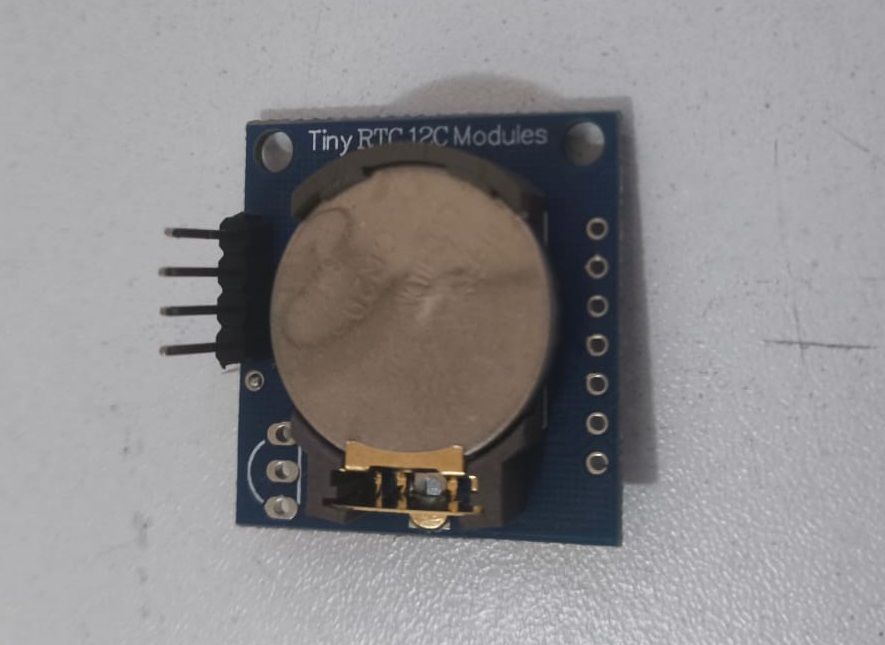
\includegraphics[width=0.6\textwidth]{Figuras/rtc.jpeg}
    \caption{Módulo RTC DS1307 utilizado no protótipo.}
    \label{fig:rtc}
    \fonte{Autor (2026).}
\end{figure}

O DS1307 comunica-se com o Arduino por meio do protocolo I\textsuperscript{2}C, utilizando as linhas SDA e SCL para troca de dados. O módulo possui bateria de backup, responsável por manter a contagem de data e hora mesmo na ausência de alimentação elétrica, preservando as informações temporais armazenadas \cite{maxim2015}.

No sistema desenvolvido, o RTC desempenhou duas funções principais. A primeira foi fornecer a referência temporal utilizada pelo algoritmo de controle para determinar o posicionamento angular do painel fotovoltaico ao longo do dia. A segunda consistiu em registrar a data e o horário correspondentes a cada medição de tensão, corrente e potência armazenada no cartão microSD, permitindo organizar os dados experimentais em ordem cronológica.

A utilização do módulo RTC garantiu a sincronização entre o controle do posicionamento do painel e a aquisição das grandezas elétricas, contribuindo para a consistência dos dados utilizados na comparação entre o sistema automatizado, o sistema de painel fixo e o modelo computacional desenvolvido neste trabalho.

\subsection{Display de Cristal Líquido (Liquid Crystal Display -- LCD)}

Para a interface entre o sistema embarcado e o usuário, foi utilizado um display LCD 16$\times$2 com interface I2C, apresentado na Figura~\ref{fig:lcd}. Esse dispositivo permite a exibição de caracteres alfanuméricos distribuídos em duas linhas de 16 colunas e é amplamente empregado em sistemas embarcados devido ao seu baixo custo, reduzido consumo de energia e facilidade de integração com microcontroladores \cite{makerhero2022}.

\begin{figure}[H]
    \centering
    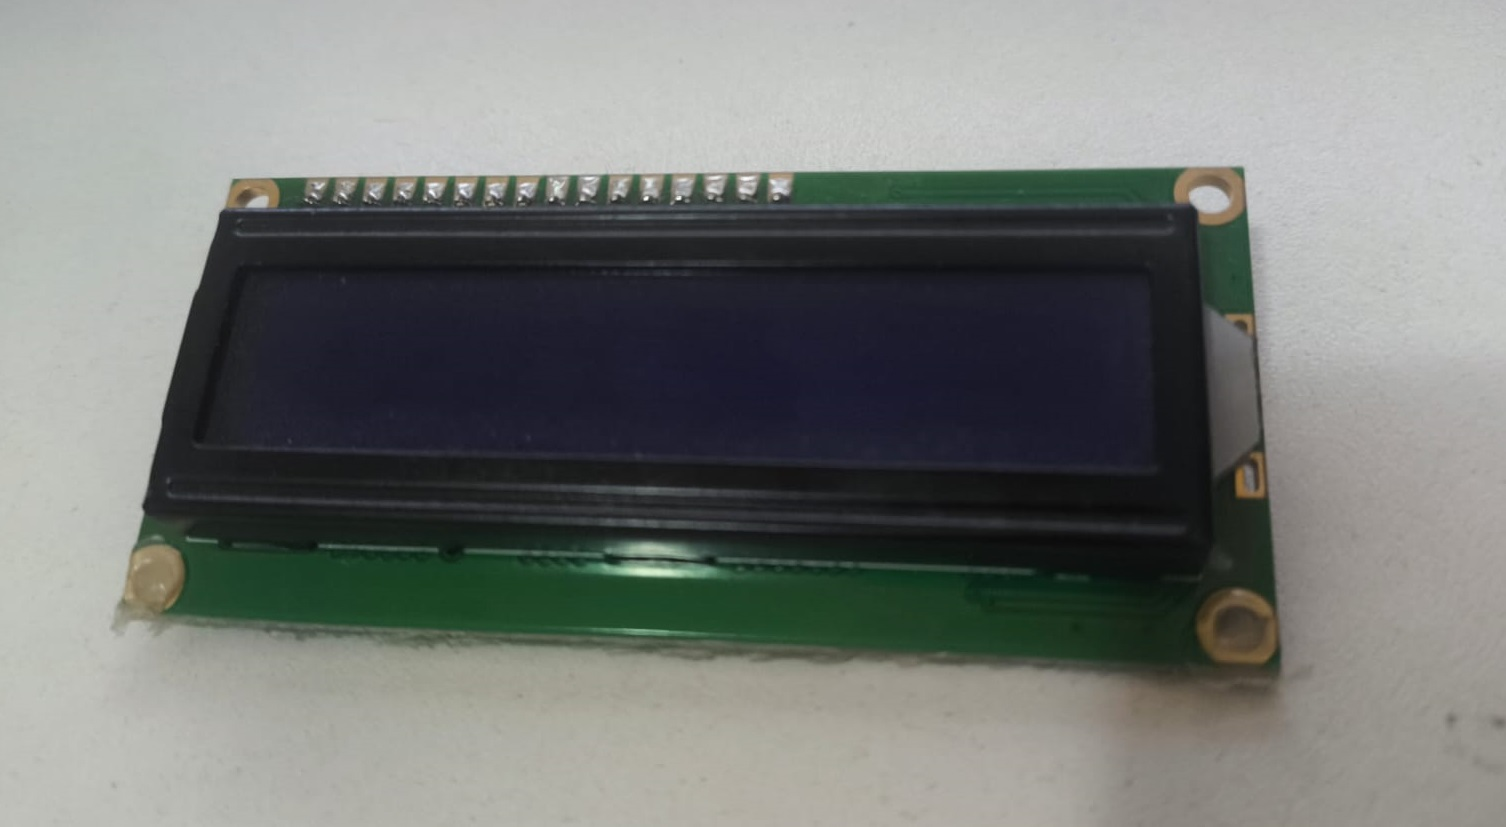
\includegraphics[width=0.6\textwidth]{Figuras/display.jpeg}
    \caption{Display LCD 16$\times$2 com interface I2C utilizado no sistema.}
    \label{fig:lcd}
    \fonte{Autor (2026).}
\end{figure}

A comunicação entre o display e o Arduino é realizada por meio do protocolo I2C, utilizando apenas as linhas SDA e SCL. Essa característica reduz a quantidade de conexões necessárias em relação à interface paralela convencional, simplificando a montagem do circuito e liberando portas de entrada e saída do microcontrolador para outras funções do sistema.

Durante a operação do protótipo, o display apresenta em tempo real as principais informações monitoradas pelo sistema, incluindo data e horário fornecidos pelo módulo RTC, tensão elétrica (V), corrente elétrica (I), potência instantânea (P) e o ângulo de posicionamento do painel fotovoltaico. Essas informações permitiram acompanhar continuamente o funcionamento do sistema durante os ensaios experimentais.

Além da exibição das variáveis elétricas, o display também foi utilizado para apresentar mensagens relacionadas ao estado de funcionamento do sistema, auxiliando no monitoramento da operação do protótipo durante a aquisição dos dados experimentais.

\subsection{Módulo Leitor de Cartão Micro SD}

Para o armazenamento dos dados experimentais foi utilizado um módulo leitor de cartão microSD, apresentado na Figura~\ref{fig:sd}. Esse dispositivo permite registrar automaticamente as informações adquiridas pelo sistema durante os ensaios, possibilitando sua utilização nas etapas de tratamento, análise e comparação dos resultados.

\begin{figure}[H]
    \centering
    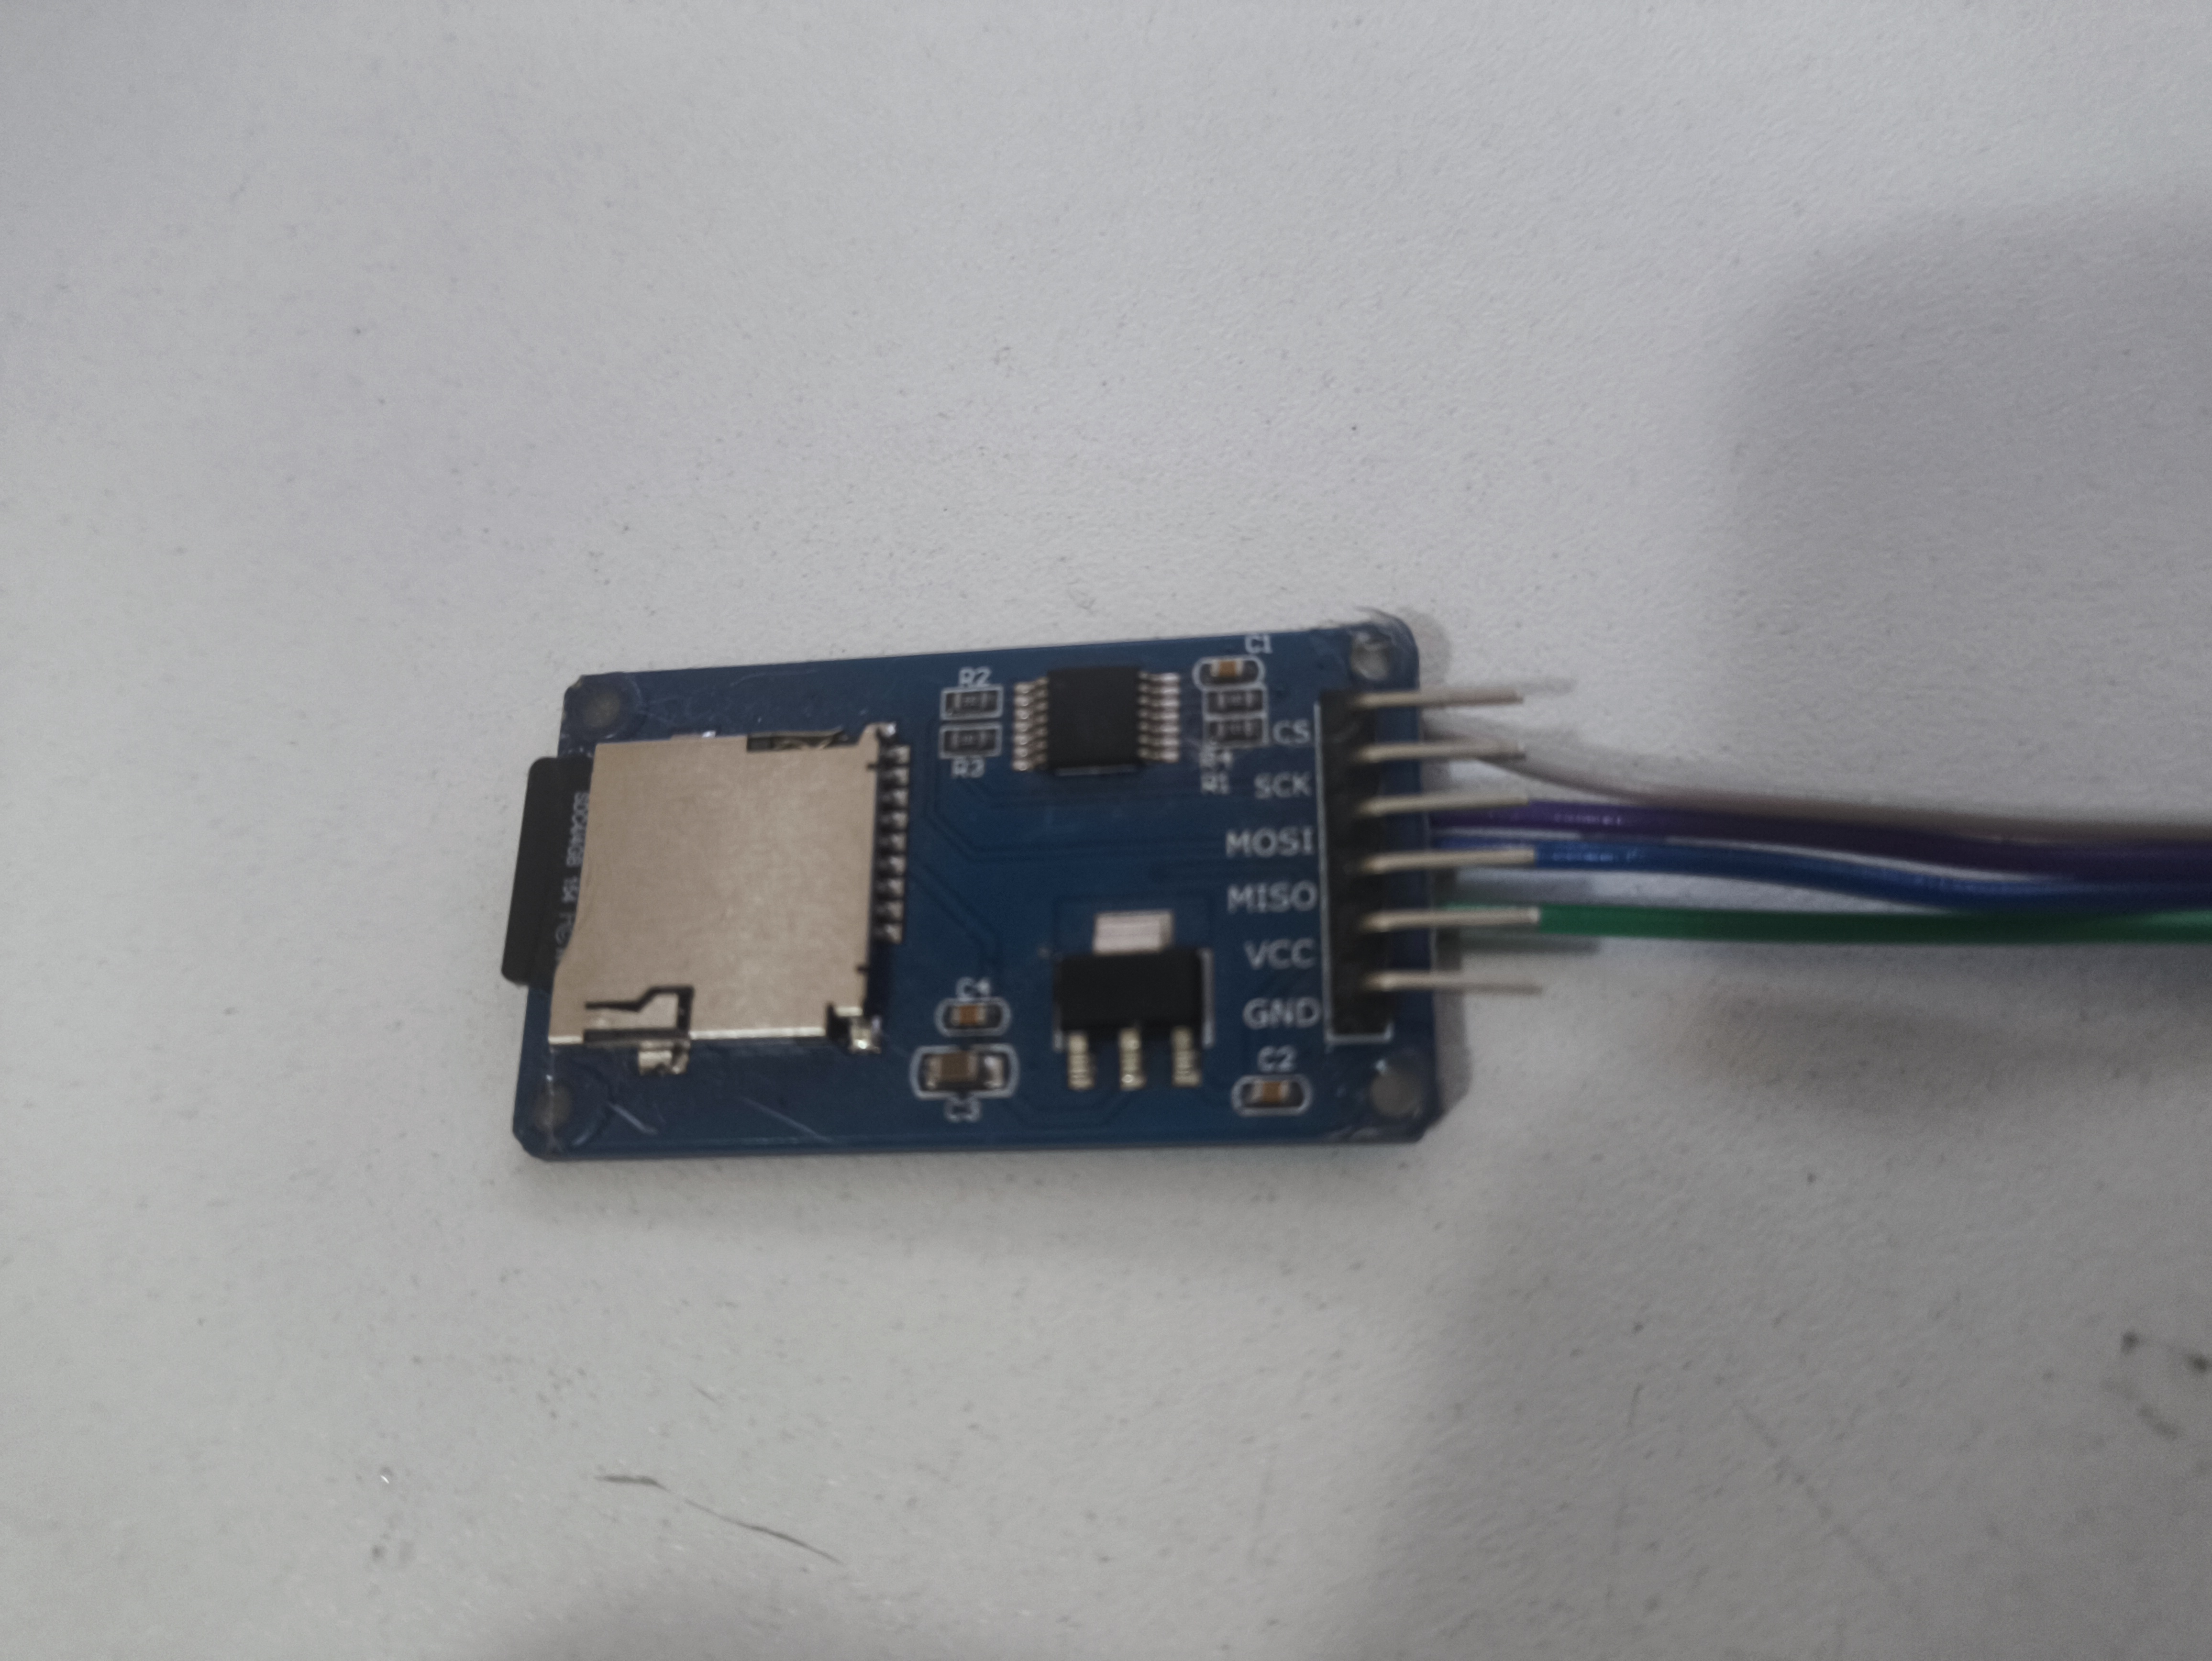
\includegraphics[width=0.6\textwidth]{Figuras/cartao_sd.jpg}
    \caption{Módulo leitor de cartão microSD utilizado no sistema.}
    \label{fig:sd}
    \fonte{Autor (2026).}
\end{figure}

O módulo comunica-se com o Arduino por meio da interface SPI (\textit{Serial Peripheral Interface}), permitindo operações de leitura e escrita em cartões de memória microSD. Essa solução é amplamente utilizada em sistemas embarcados que necessitam registrar dados durante longos períodos de operação, possibilitando o armazenamento organizado das informações em arquivos digitais compatíveis com softwares de planilhas eletrônicas e ferramentas de análise de dados \cite{eletrogate2022}.

No protótipo desenvolvido, foram registrados automaticamente a data, o horário, a tensão elétrica, a corrente elétrica, a potência instantânea e o ângulo de posicionamento do painel fotovoltaico. O registro cronológico dessas informações permitiu a construção das séries temporais utilizadas na comparação entre o sistema automatizado e o sistema de painel fixo.

Após a realização dos experimentos, os arquivos foram importados para planilhas eletrônicas, onde os dados foram organizados e processados para obtenção dos gráficos, tabelas e indicadores utilizados na análise dos resultados.

Dessa forma, o módulo leitor de cartão microSD desempenhou papel fundamental no sistema de aquisição de dados, garantindo o registro organizado das informações experimentais e fornecendo suporte às etapas de processamento, análise e validação dos resultados obtidos.

\subsection{Arquitetura do Sistema}

A arquitetura do protótipo foi desenvolvida para possibilitar a aquisição de dados experimentais destinados à validação do modelo computacional e à comparação do desempenho entre um sistema fotovoltaico automatizado e um sistema de painel fixo. Dessa forma, o protótipo constitui uma ferramenta de pesquisa destinada à aquisição de dados experimentais, não representando um sistema projetado para aplicação comercial ou operação contínua em ambientes externos.

A estrutura do protótipo foi construída utilizando uma base de madeira e componentes mecânicos fabricados por impressão 3D em filamento PLA, incluindo o suporte do painel fotovoltaico e o conjunto de engrenagens responsável pela transmissão do movimento. A opção por esses materiais deve-se ao baixo custo e à facilidade de fabricação, características adequadas ao desenvolvimento de protótipos acadêmicos. Entretanto, reconhece-se que os materiais apresentam limitações quanto à resistência mecânica e à durabilidade quando expostos continuamente às condições ambientais, como radiação ultravioleta, variações de temperatura e intempéries. Assim, o protótipo foi concebido exclusivamente para a realização dos testes experimentais previstos neste trabalho.

A movimentação do painel fotovoltaico é realizada por um servomotor MG996R acoplado ao conjunto de engrenagens impressas em PLA, permitindo a rotação do painel em torno de um único eixo no sentido leste-oeste. Essa configuração reproduz o princípio de funcionamento de um sistema de rastreamento solar de eixo único, sendo suficiente para os experimentos realizados. Como o objetivo deste trabalho consiste na validação do modelo computacional por meio de dados experimentais, não foram avaliados aspectos relacionados à resistência mecânica ou à viabilidade construtiva do protótipo.

As Figuras~\ref{fig:engrenagem1} e~\ref{fig:engrenagem2} apresentam o suporte estrutural e o conjunto de engrenagens utilizados no sistema de transmissão mecânica.

\begin{figure}[H]
    \centering
    \begin{minipage}{0.45\linewidth}
        \centering
        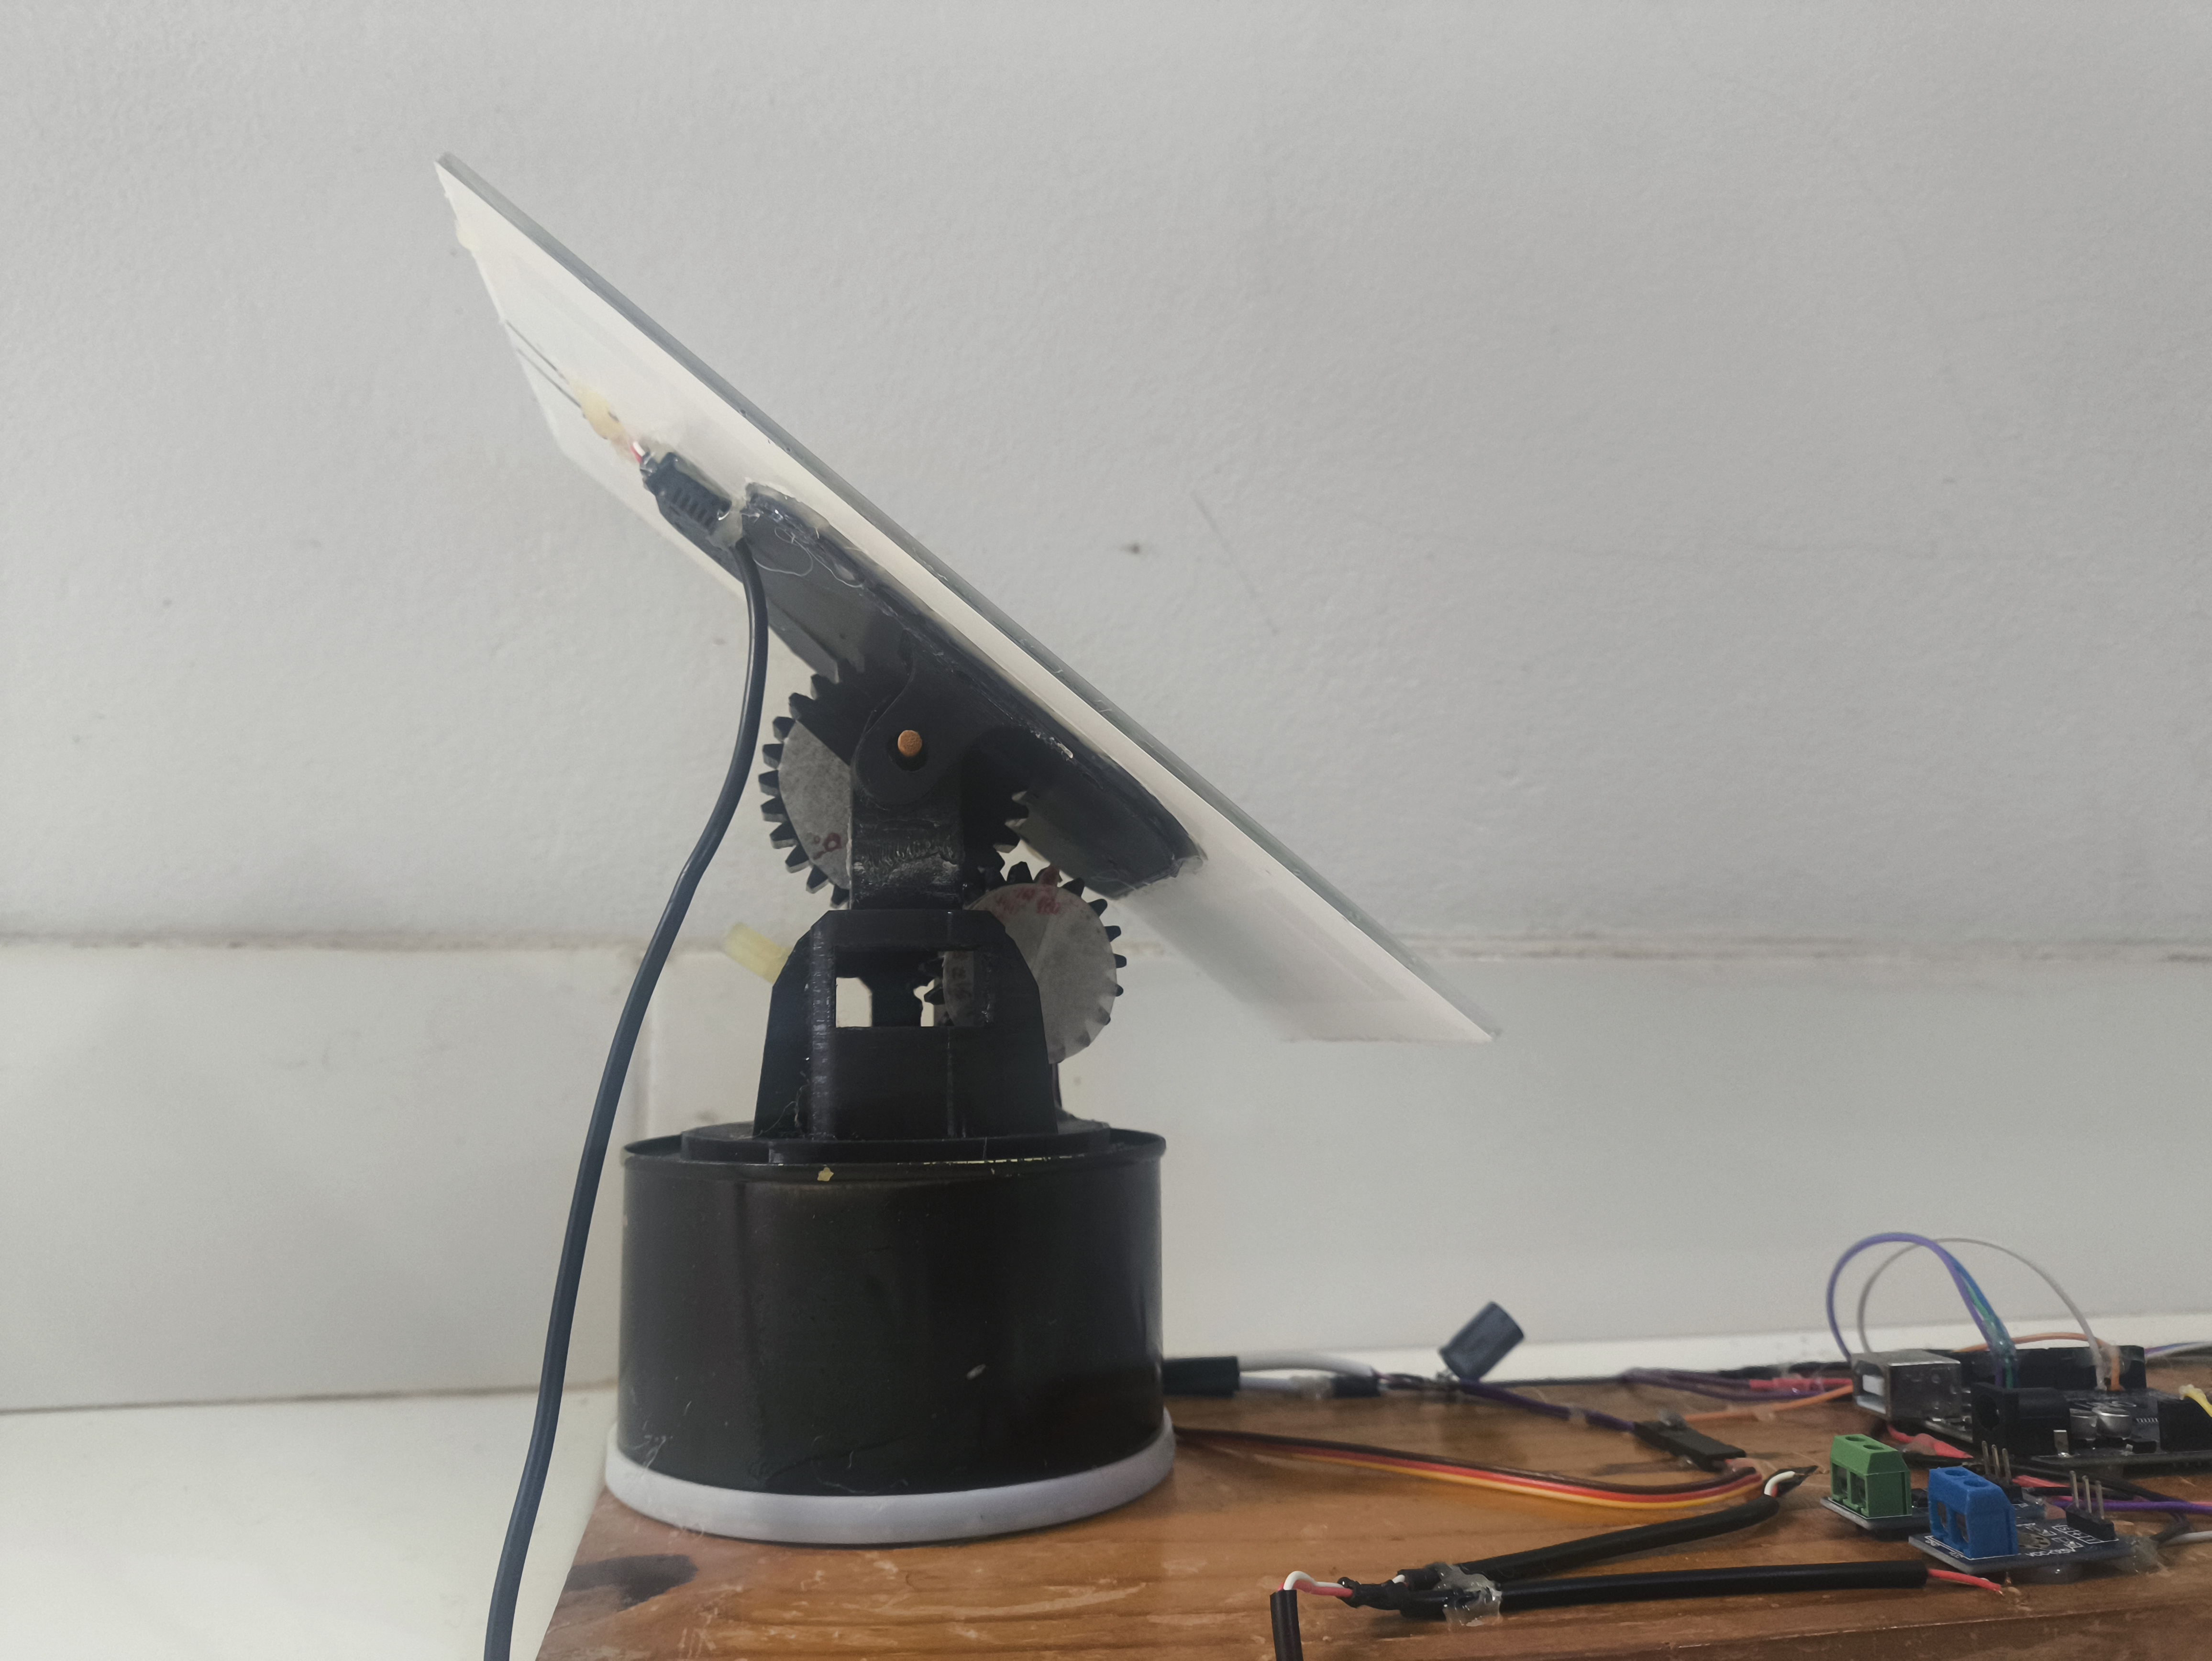
\includegraphics[width=\linewidth]{Figuras/engrenagem1.jpg}
        \caption{Suporte e engrenagem produzidos por impressão 3D.}
        \label{fig:engrenagem1}
        \fonte{Autor (2026).}
    \end{minipage}
    \hfill
    \begin{minipage}{0.45\linewidth}
        \centering
        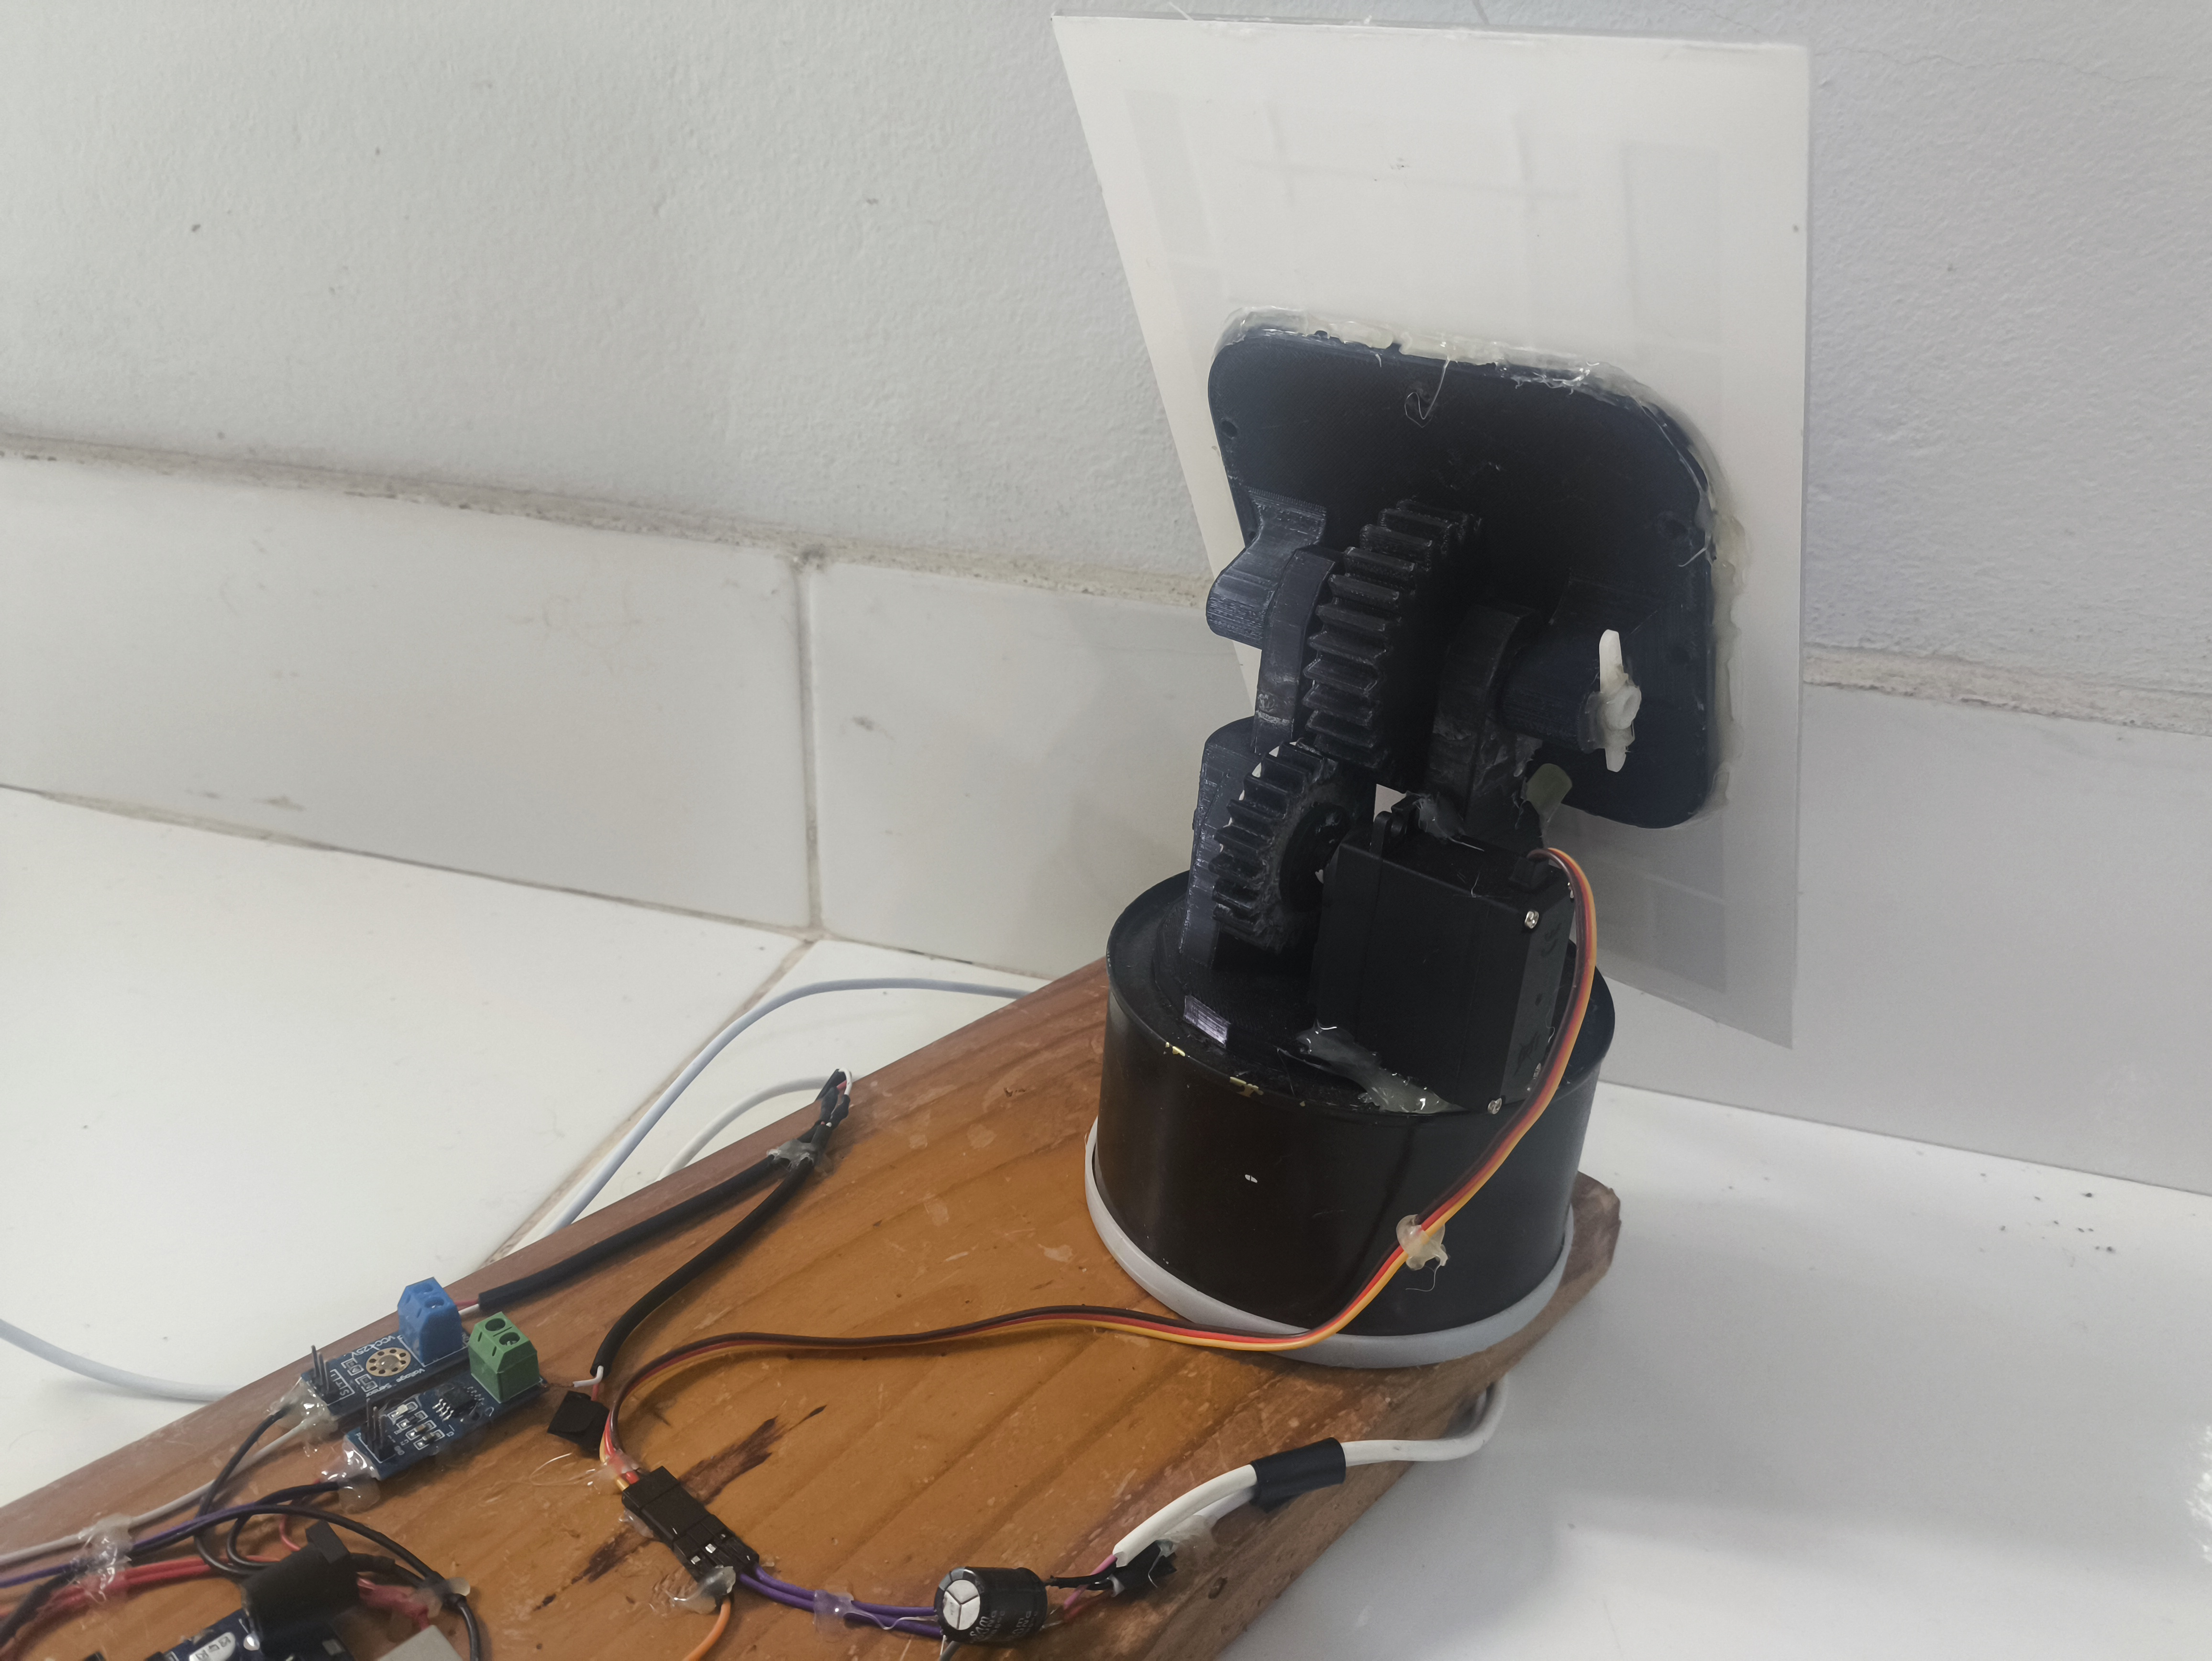
\includegraphics[width=\linewidth]{Figuras/engrenagem2.jpg}
        \caption{Detalhamento do conjunto de transmissão mecânica.}
        \label{fig:engrenagem2}
        \fonte{Autor (2026).}
    \end{minipage}
\end{figure}

Os componentes eletrônicos, incluindo o Arduino Uno, os sensores, o módulo RTC, o display LCD e o módulo leitor de cartão microSD, foram organizados sobre a base estrutural de forma a facilitar a montagem, a manutenção e a organização das conexões elétricas, contribuindo para a confiabilidade durante os ensaios experimentais.

A Figura~\ref{fig:prototipo_montado} apresenta o protótipo completamente montado, evidenciando a integração entre a estrutura mecânica, o sistema de acionamento e os módulos eletrônicos utilizados no desenvolvimento do trabalho.

\begin{figure}[H]
    \centering
    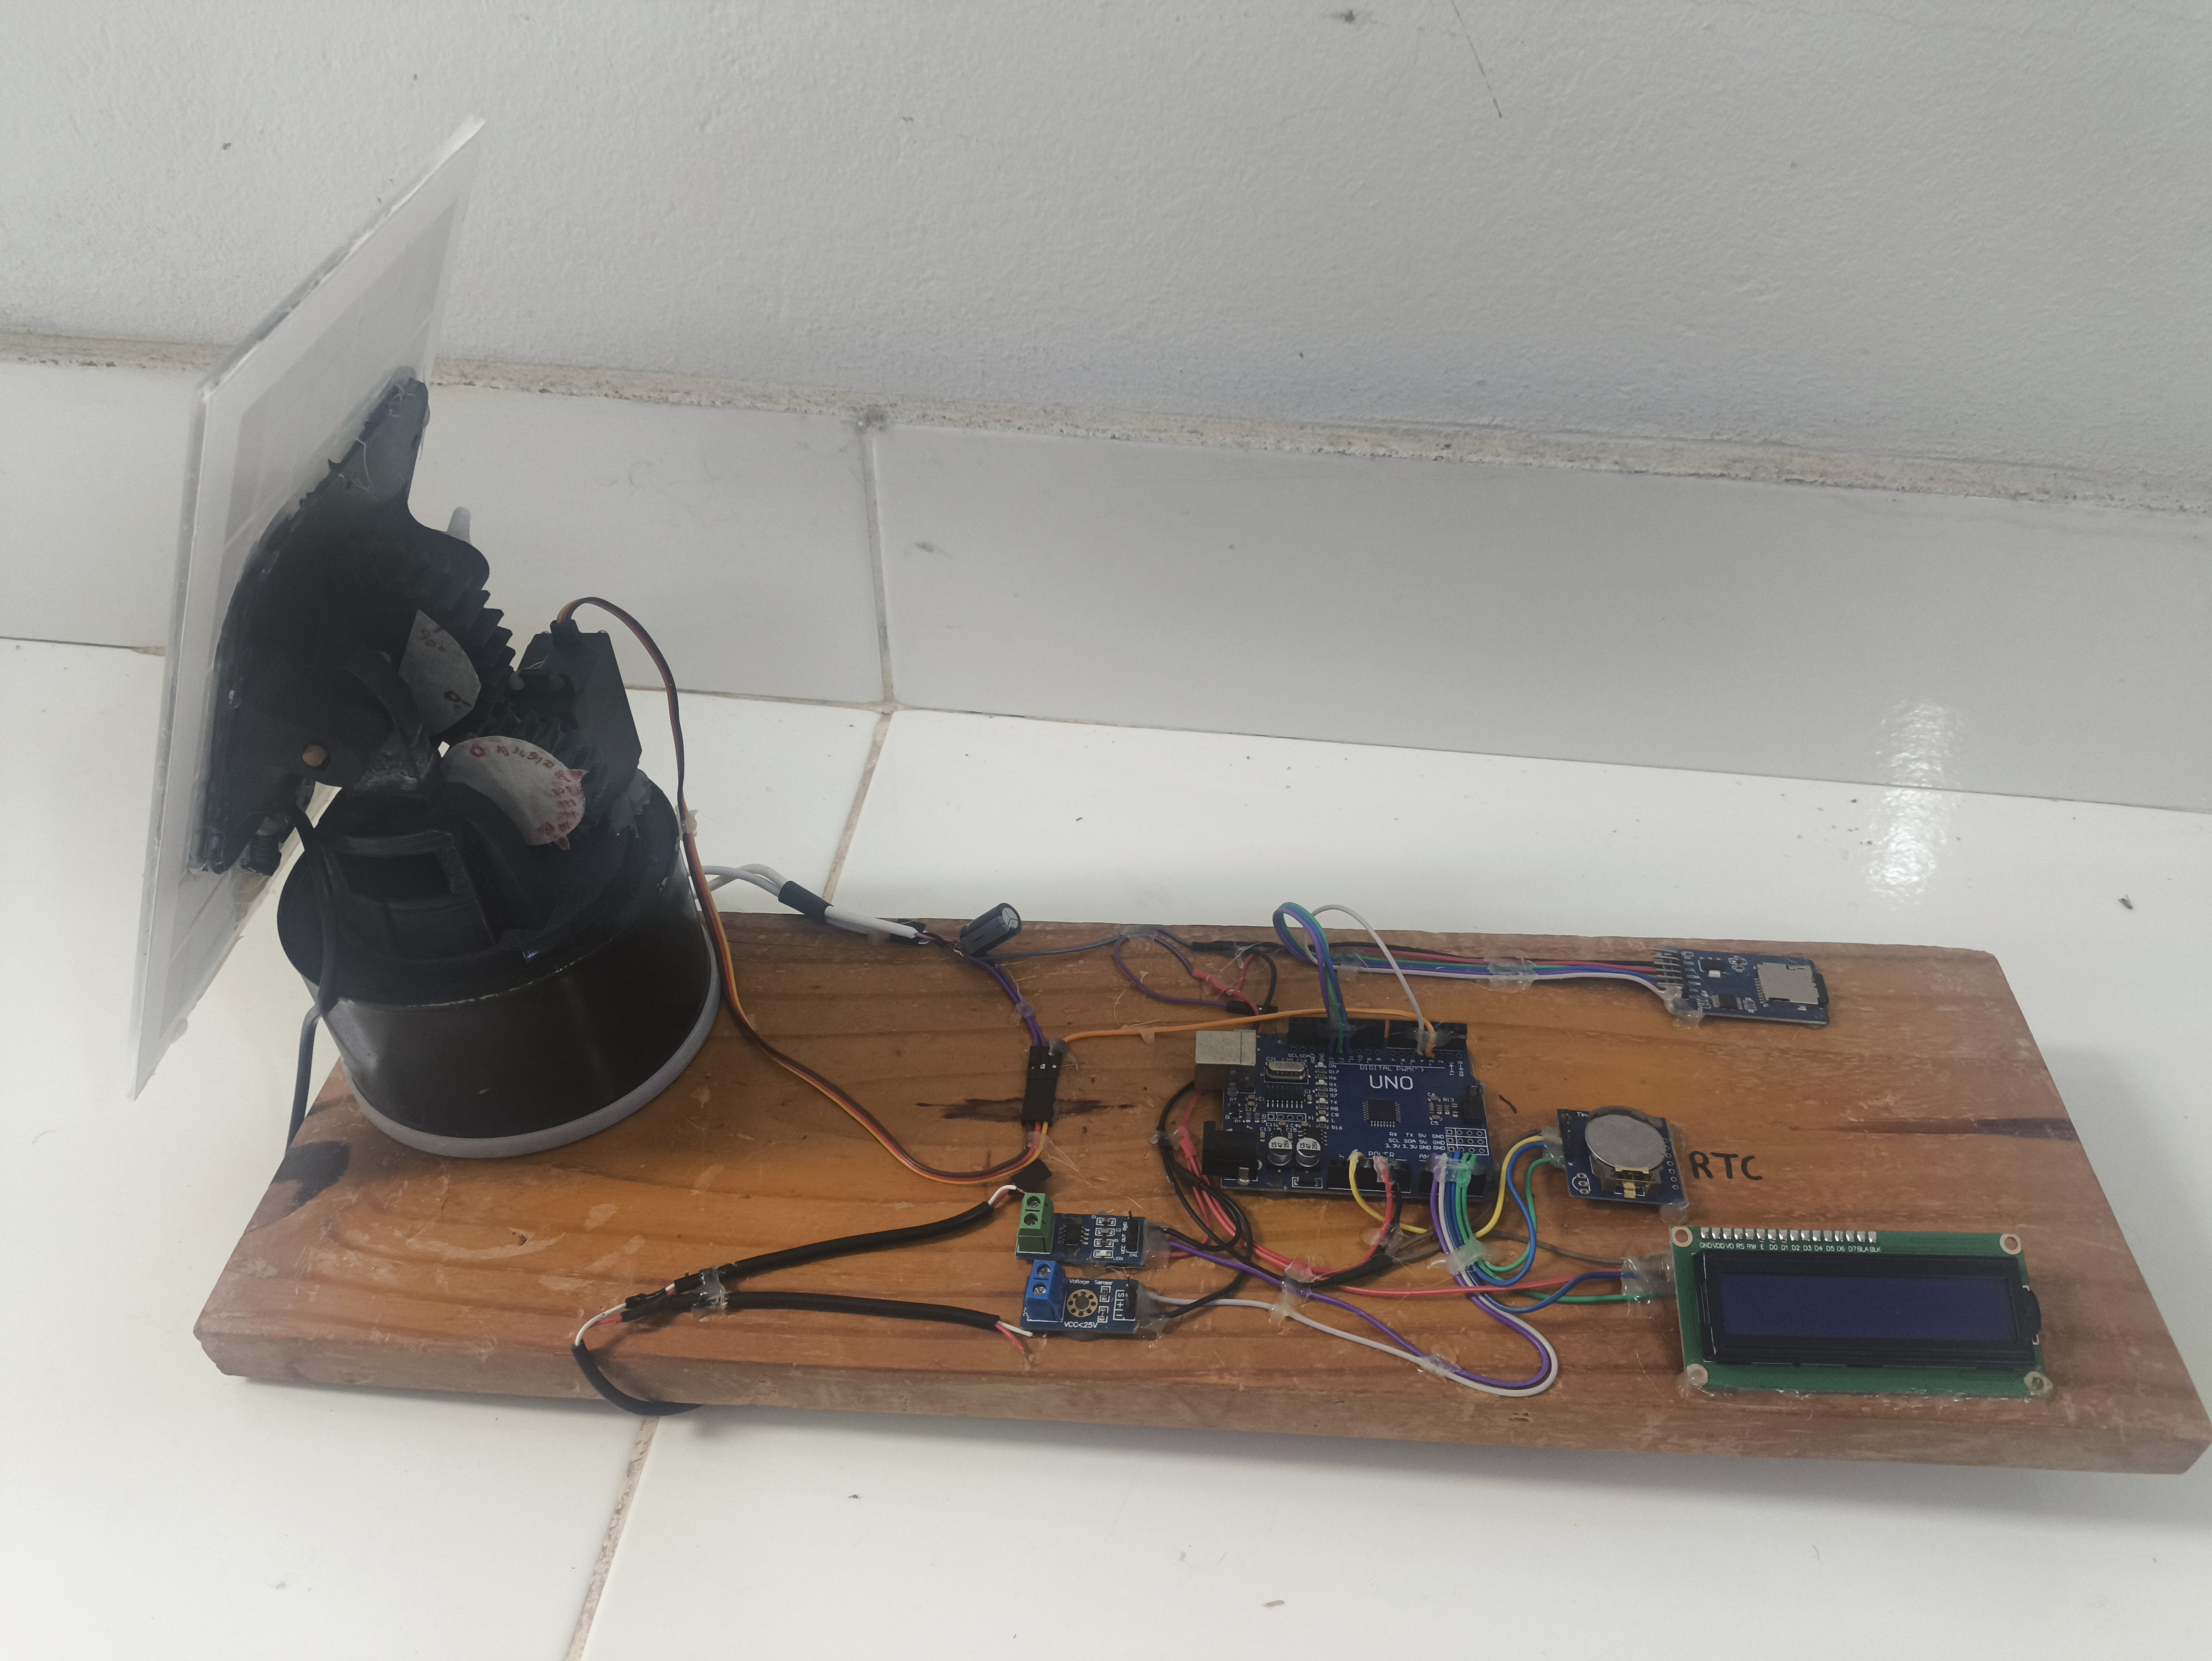
\includegraphics[width=0.6\linewidth]{Figuras/prototipo_montado.jpg}
    \caption{Protótipo do sistema automatizado desenvolvido.}
    \label{fig:prototipo_montado}
    \fonte{Autor (2026).}
\end{figure}

Como os ensaios foram realizados em ambiente externo, foi construída uma estrutura de proteção destinada a minimizar a exposição dos componentes eletrônicos à chuva, à umidade, à radiação solar direta, à poeira e a outros agentes externos, preservando a integridade do sistema durante a coleta de dados.

A estrutura de proteção construída é apresentada na Figura~\ref{fig:protecao_prototipo}.

\begin{figure}[H]
    \centering
    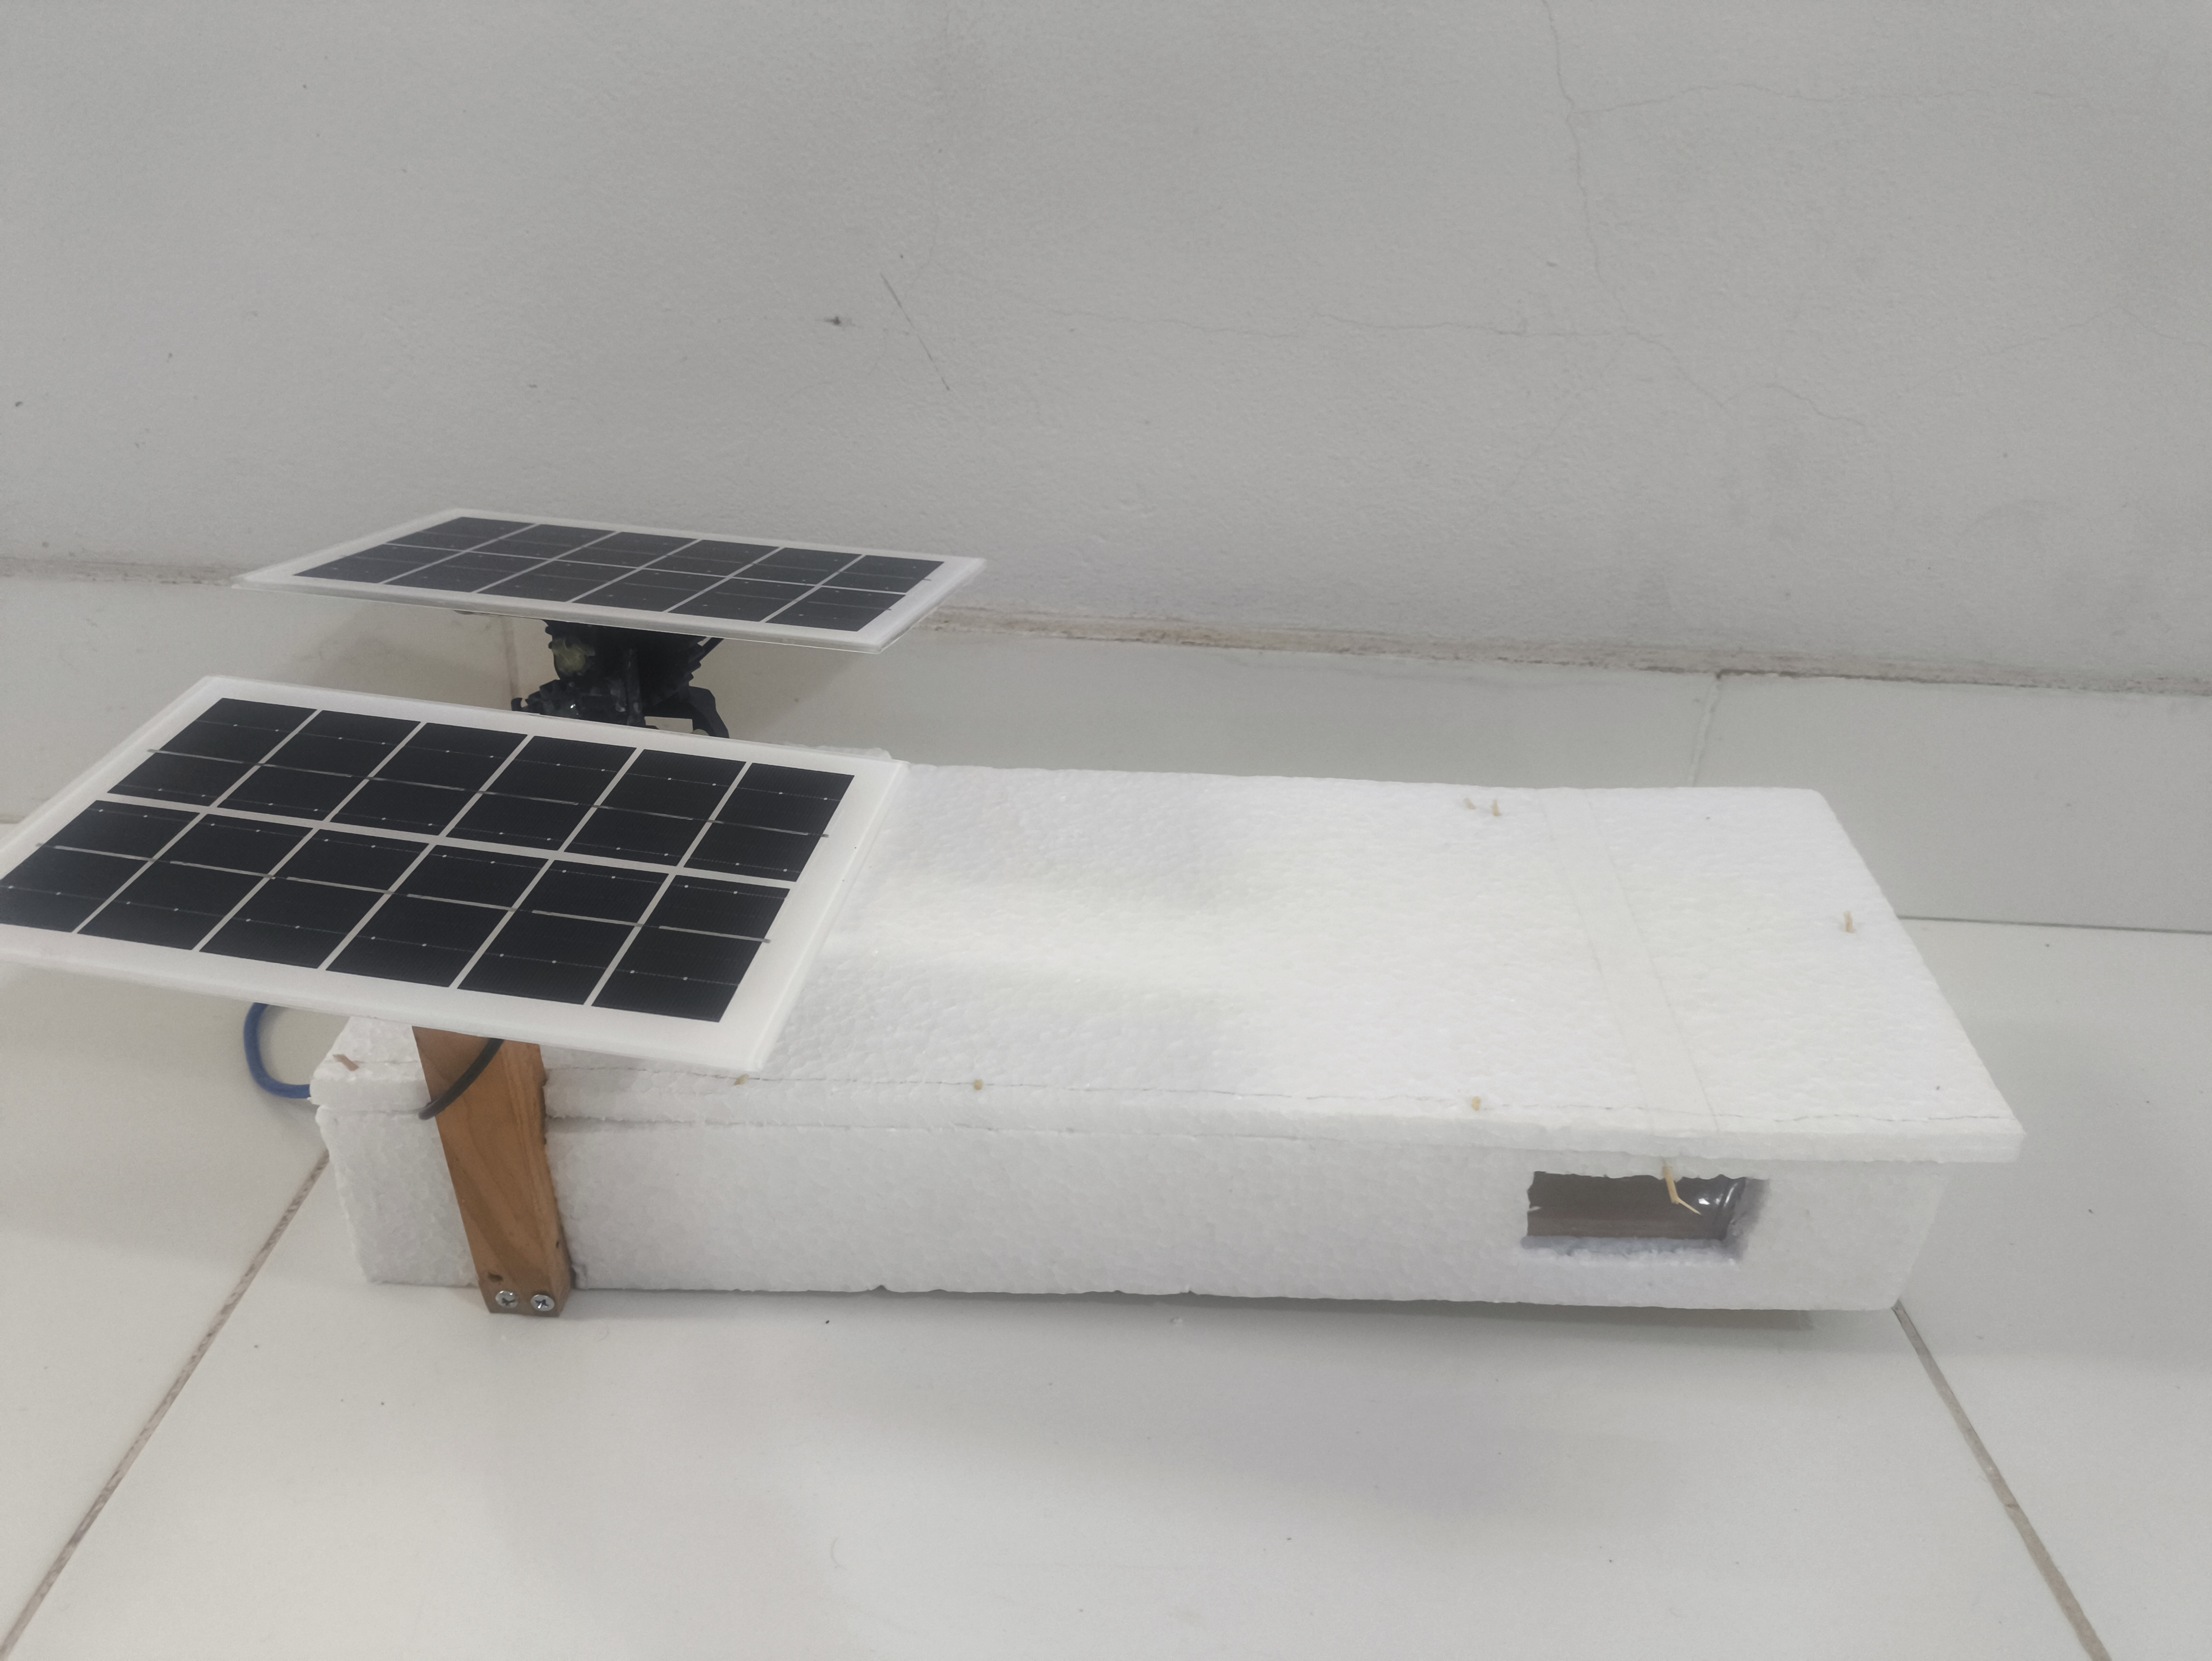
\includegraphics[width=0.7\linewidth]{Figuras/proteçao_prototipo.jpg}
    \caption{Estrutura de proteção do protótipo durante os experimentos.}
    \label{fig:protecao_prototipo}
    \fonte{Autor (2026).}
\end{figure}

A integração entre a estrutura mecânica, o sistema de acionamento e os módulos eletrônicos resultou em um protótipo capaz de realizar automaticamente o posicionamento do painel fotovoltaico, a aquisição das grandezas elétricas e o armazenamento das medições. Esse protótipo constituiu a plataforma experimental utilizada para gerar os dados empregados na validação do modelo computacional e na comparação entre os sistemas automatizado e de painel fixo.

\section{Lógica de Funcionamento do Sistema}

O funcionamento do sistema embarcado foi implementado por meio de um algoritmo de controle responsável por integrar a aquisição de dados, o posicionamento automatizado do painel fotovoltaico, o cálculo das grandezas elétricas e o armazenamento das informações experimentais. O algoritmo foi desenvolvido para operar continuamente durante o período de funcionamento do sistema, permitindo a execução automática das etapas de monitoramento, controle e registro dos dados utilizados na validação do modelo computacional.

A lógica de funcionamento baseia-se na utilização das informações de data e horário fornecidas pelo módulo RTC para determinar o posicionamento do painel fotovoltaico ao longo do dia. Além disso, são realizados pequenos ajustes no posicionamento a partir da potência elétrica medida, com o objetivo de corrigir eventuais diferenças entre a posição teórica e a condição de maior geração de energia.

As subseções seguintes apresentam o fluxograma do algoritmo e descrevem detalhadamente as principais etapas de funcionamento implementadas no sistema embarcado.

\subsection{Fluxograma do Algoritmo}

A lógica de funcionamento do sistema foi implementada no microcontrolador Arduino, responsável por executar as rotinas de inicialização, aquisição de dados, controle do posicionamento do painel fotovoltaico e armazenamento das informações coletadas.

O algoritmo foi desenvolvido de forma sequencial, integrando a leitura do módulo RTC, a determinação do ângulo de posicionamento, o acionamento do servomotor, a aquisição das variáveis elétricas e o registro dos dados em cartão microSD. A Figura~\ref{fig:fluxograma} apresenta o fluxograma simplificado do algoritmo implementado no sistema embarcado.

\begin{figure}[htbp]
\centering
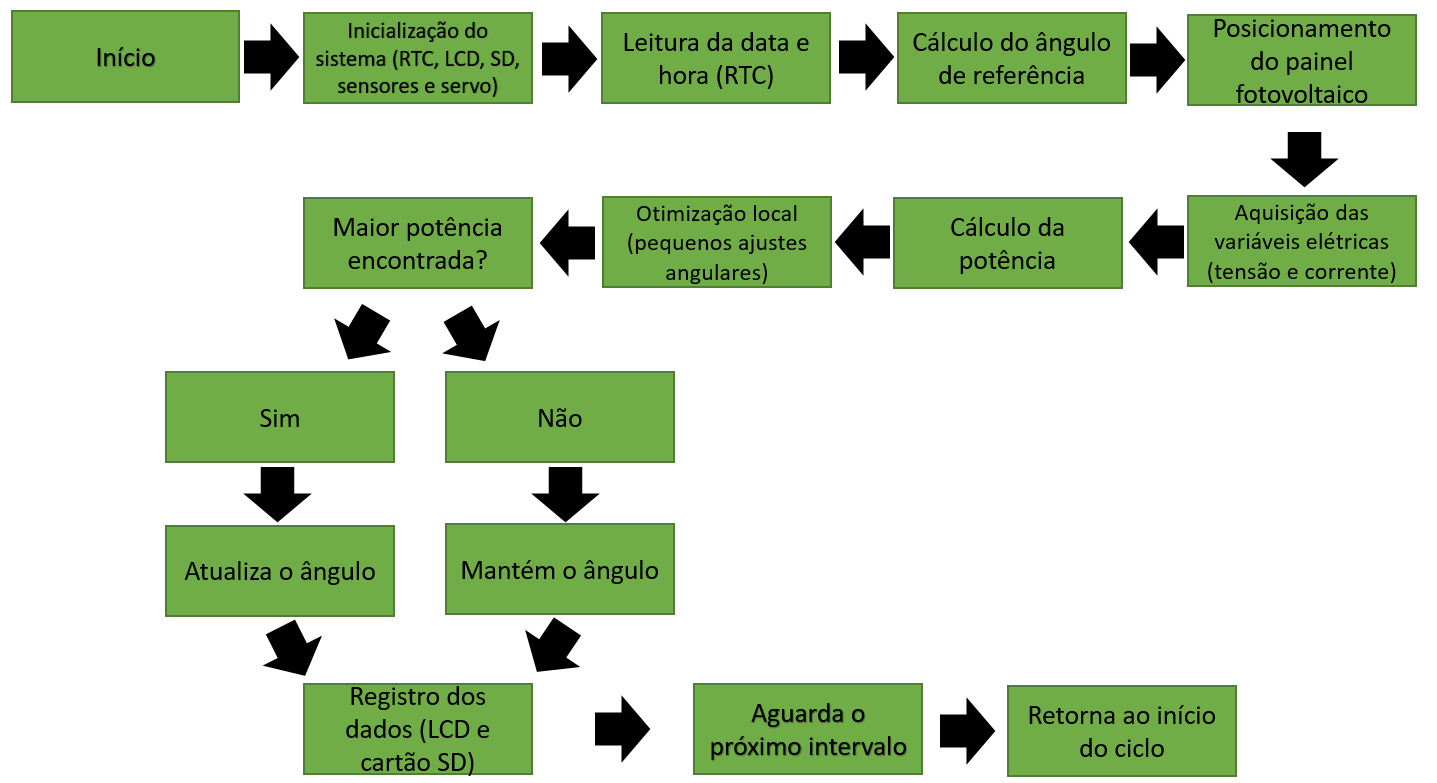
\includegraphics[width=0.90\textwidth]{Figuras/fluxograma_algoritimo.png}
\caption{Fluxograma do algoritmo de controle implementado no sistema automatizado.}
\label{fig:fluxograma}
\fonte{Autor (2026).}
\end{figure}

O algoritmo inicia com a configuração dos módulos de comunicação, dos sensores, do servomotor, do display LCD, do módulo RTC e do cartão microSD. Após essa etapa, entra em um ciclo contínuo de execução durante o período de funcionamento do sistema.

Inicialmente, são obtidas a data e a hora fornecidas pelo módulo RTC. Com base nessas informações, é determinado o ângulo de referência correspondente ao horário atual, utilizado como posição inicial do painel fotovoltaico.

Na sequência, são realizadas as leituras dos sensores de tensão e corrente, permitindo o cálculo da potência elétrica instantânea produzida pelo painel fotovoltaico.

Em seguida, é executada uma rotina de ajuste fino do posicionamento, na qual são realizados pequenos deslocamentos angulares em torno da posição de referência, comparando-se a potência elétrica obtida em cada posição. Ao final dessa etapa, o painel é reposicionado no ângulo que apresentou a maior potência medida.

Após a definição da posição final, os valores de tensão, corrente, potência, ângulo, data e horário são apresentados no display LCD e registrados automaticamente no cartão microSD. Em seguida, o algoritmo reinicia o ciclo de operação, repetindo essa sequência durante todo o período de funcionamento do sistema.

\subsection{Controle do Servo Motor}

O posicionamento do painel fotovoltaico é realizado por um servomotor MG996R, acionado pelo microcontrolador Arduino Uno por meio de sinais PWM (\textit{Pulse Width Modulation}). Nessa técnica, a largura do pulso determina a posição angular do eixo do servomotor, permitindo controlar a orientação do painel ao longo do dia.

A estratégia de controle desenvolvida neste trabalho combina um modelo temporal com uma etapa de ajuste baseada na potência elétrica gerada pelo painel fotovoltaico. Inicialmente, o módulo RTC DS1307 fornece ao microcontrolador as informações de data e horário. A partir desses dados, é calculado o ângulo de referência do painel por meio de uma interpolação linear entre os horários de início e término da operação do sistema, conforme a Equação~\ref{eq:angulo}.

\begin{equation}
\theta=\theta_i+\left(\frac{t-t_i}{t_f-t_i}\right)(\theta_f-\theta_i)
\label{eq:angulo}
\end{equation}

em que $\theta$ representa o ângulo de referência do painel, $\theta_i$ e $\theta_f$ correspondem aos ângulos inicial e final do sistema, respectivamente, enquanto $t$ representa o horário atual fornecido pelo RTC, sendo $t_i$ e $t_f$ os horários de início e término da operação.

Após posicionar o painel no ângulo de referência, o algoritmo executa, a cada 10 minutos, uma rotina de ajuste fino do posicionamento. Esse intervalo foi adotado por representar um compromisso entre a necessidade de acompanhar o deslocamento aparente do Sol e a redução do número de acionamentos do servomotor, minimizando o desgaste mecânico e o consumo de energia do sistema.

Durante essa etapa, o servomotor realiza pequenos deslocamentos angulares em torno da posição de referência, efetuando medições de tensão e corrente em cada posição avaliada. A potência elétrica instantânea é determinada por meio da Equação~\ref{eq:potencia}.

\begin{equation}
P = V \cdot I
\label{eq:potencia}
\end{equation}

em que $P$ representa a potência elétrica gerada pelo painel fotovoltaico (W), $V$ corresponde à tensão elétrica medida nos terminais do painel (V) e $I$ representa a corrente elétrica fornecida pelo módulo fotovoltaico (A).

Embora os métodos de rastreamento do ponto de máxima potência (\textit{Maximum Power Point Tracking} -- MPPT) tenham como objetivo maximizar a potência extraída dos módulos fotovoltaicos por meio do ajuste contínuo do ponto de operação elétrico do sistema \cite{esram2007}, neste trabalho não foi implementado um algoritmo MPPT. A potência elétrica medida pelos sensores foi utilizada apenas como variável de referência para realizar pequenos ajustes na orientação mecânica do painel fotovoltaico, buscando identificar a posição que proporciona a maior geração de energia.

Essa estratégia permite compensar pequenas diferenças entre a posição teórica do Sol e as condições reais de operação, como variações de irradiância, nebulosidade, desalinhamentos mecânicos e pequenas imprecisões construtivas. Ao término da rotina de ajuste, o painel é reposicionado automaticamente no ângulo correspondente ao maior valor de potência medido.

Ao final de cada ciclo de controle, o microcontrolador registra automaticamente no cartão microSD as informações de data, horário, tensão, corrente, potência e ângulo de posicionamento do painel. Simultaneamente, essas variáveis são apresentadas em tempo real no display LCD, permitindo o acompanhamento contínuo da operação do sistema durante os ensaios experimentais.

A Figura~\ref{fig:esquema} apresenta a integração entre o microcontrolador, o servomotor e os demais dispositivos utilizados no sistema de controle.

\begin{figure}[H]
    \centering
    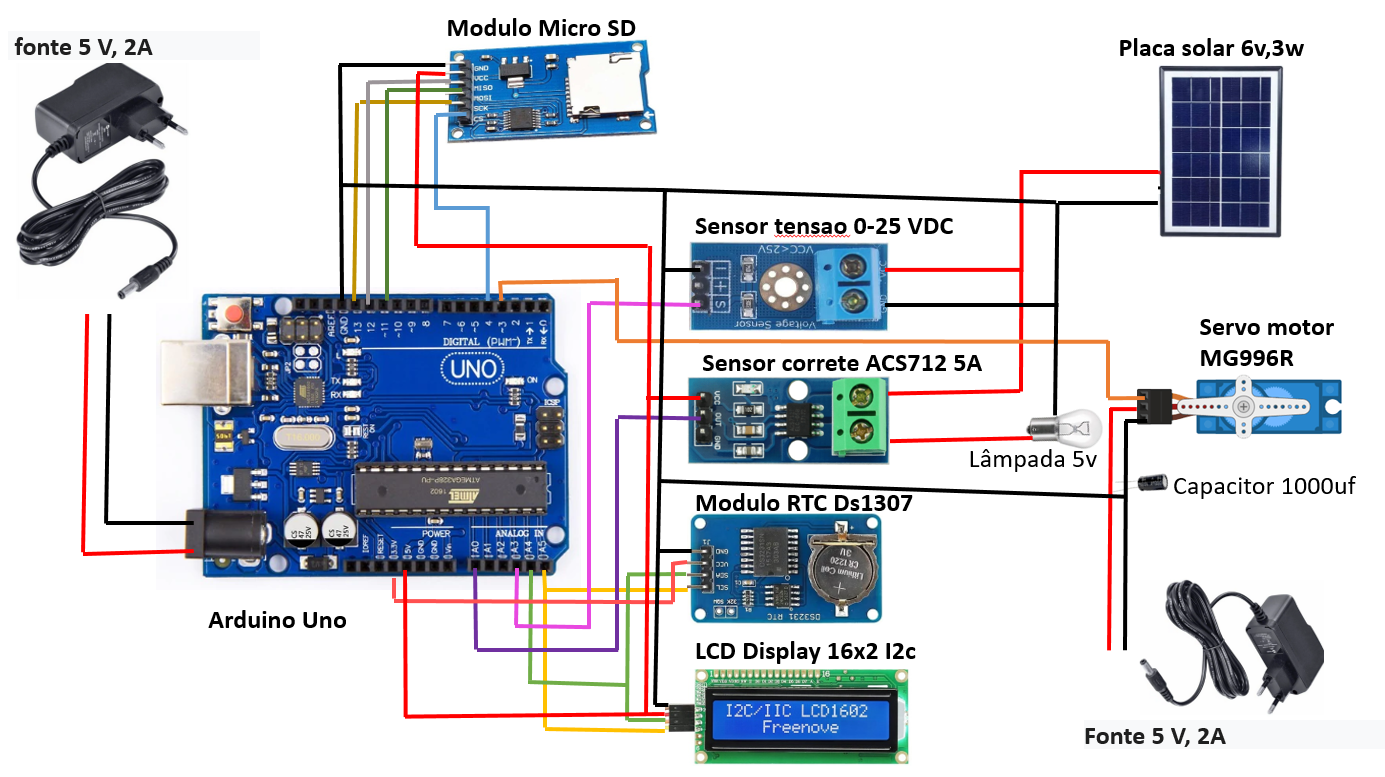
\includegraphics[width=0.9\textwidth]{Figuras/esquema.png}
    \caption{Integração entre o microcontrolador, o servomotor e os demais módulos do sistema.}
    \label{fig:esquema}
    \fonte{Autor (2026).}
\end{figure}

\subsection{Aquisição dos Dados}

A aquisição dos dados foi realizada continuamente durante o funcionamento do sistema embarcado, sendo coordenada pelo microcontrolador Arduino Uno. Após cada ciclo de posicionamento do painel fotovoltaico, o sistema realiza a leitura das grandezas elétricas por meio dos sensores de tensão e corrente, processa as informações obtidas e calcula a potência elétrica correspondente.

As leituras são realizadas pelas entradas analógicas do microcontrolador, que converte os sinais provenientes dos sensores em valores digitais por meio do conversor analógico-digital (ADC) de 10 bits. Em seguida, esses valores são convertidos para suas respectivas unidades físicas utilizando os fatores de calibração adotados para cada sensor.

A potência elétrica instantânea gerada pelo painel fotovoltaico é calculada a partir das medições de tensão e corrente, conforme a Equação~\ref{eq:potencia}.

Após o processamento das medições, o sistema associa automaticamente cada registro às informações de data e horário fornecidas pelo módulo RTC DS1307. Os dados são então armazenados automaticamente, em intervalos de um minuto, em um cartão microSD no formato texto (.txt), formando uma série temporal das variáveis monitoradas.

Cada registro contém as seguintes informações:

\begin{itemize}
    \item data da medição;
    \item horário da aquisição;
    \item tensão elétrica (V);
    \item corrente elétrica (A);
    \item potência elétrica (W);
    \item ângulo de posicionamento do painel (°).
\end{itemize}

Além do armazenamento permanente no cartão microSD, as principais variáveis monitoradas são apresentadas em tempo real no display LCD, permitindo acompanhar o funcionamento do sistema durante os ensaios experimentais. Os registros completos obtidos durante os experimentos encontram-se apresentados no Apêndice~\ref{ap:apendiceC}.

A frequência de aquisição de um minuto foi definida por representar adequadamente a variação das grandezas elétricas ao longo do período de operação, possibilitando a obtenção de uma base de dados representativa sem gerar um volume excessivo de registros. Os dados coletados foram posteriormente utilizados na análise do desempenho do sistema automatizado e na validação do modelo computacional desenvolvido no ambiente MATLAB/Simulink.

\section{Modelagem e Simulação Computacional}
\label{sec:modelagem_simulacao}

A modelagem computacional constituiu uma etapa fundamental deste trabalho, sendo utilizada para representar o comportamento do sistema fotovoltaico automatizado e possibilitar sua comparação com os resultados obtidos experimentalmente. Dessa forma, o modelo desenvolvido serviu como base para a validação da capacidade da simulação em representar o comportamento observado no protótipo físico.

O modelo computacional foi implementado no ambiente MATLAB/Simulink a partir do trabalho disponibilizado por Nagi (\citeyear{nagi2023}), sendo realizadas adaptações para representar as características do sistema desenvolvido nesta pesquisa. A partir desse modelo, foram simulados um sistema fotovoltaico automatizado e um sistema com painel fixo, permitindo comparar seu desempenho energético com os resultados experimentais obtidos durante os ensaios realizados.

As subseções seguintes apresentam a modelagem matemática adotada, o desenvolvimento do modelo computacional no ambiente MATLAB/Simulink e o procedimento utilizado para sua validação por meio da comparação entre os resultados simulados e os dados experimentais obtidos com o protótipo físico.

A trajetória aparente do Sol foi representada por uma função senoidal, utilizada para reproduzir qualitativamente a variação diária da incidência da radiação solar sobre o painel fotovoltaico. Essa aproximação permite representar o comportamento do sistema ao longo do período de simulação sem recorrer a modelos astronômicos mais complexos.

\begin{equation}
S(t)=\sin\left(\frac{\pi t}{12}\right)
\label{eq:trajetoria}
\end{equation}

em que S(t) representa a posição relativa do Sol ao longo do dia e t corresponde ao tempo de simulação, expresso em horas.

Para representar a irradiância incidente sobre o painel, o modelo considera uma componente direta e uma componente difusa. Na implementação realizada foram adotados valores constantes de 900 W/m² para a irradiância direta máxima e 100 W/m² para a irradiância difusa, totalizando aproximadamente 1000 W/m² nas condições de máxima incidência, valor compatível com as Condições Padrão de Teste (STC).

No sistema automatizado, a potência simulada é considerada proporcional à irradiância incidente sobre o painel. Para o sistema com painel fixo, foi introduzido um fator angular que reduz a parcela da irradiância direta recebida pelo módulo em função do desalinhamento entre o painel e a posição aparente do Sol. Dessa forma, o sistema fixo apresenta menor geração de potência durante parte do período de operação quando comparado ao sistema automatizado.

A energia produzida por cada configuração foi obtida por meio da integração da potência ao longo do tempo, conforme a Equação~\ref{eq:energia}.

\begin{equation}
E=\int P(t),dt
\label{eq:energia}
\end{equation}

em que E representa a energia acumulada e P(t) corresponde à potência instantânea produzida pelo sistema.

O ganho percentual do sistema automatizado em relação ao sistema com painel fixo foi determinado pela Equação~\ref{eq:ganho}.

\begin{equation}
G(%)=
\frac{E_{aut}-E_{fixo}}
{E_{fixo}}
\times100
\label{eq:ganho}
\end{equation}

em que $E_{aut}$ representa a energia produzida pelo sistema automatizado e $E_{fixo}$ representa a energia produzida pelo sistema com painel fixo.

No protótipo físico, a potência elétrica foi determinada experimentalmente a partir das medições de tensão e corrente realizadas pelos sensores instalados no sistema, utilizando a Equação~\ref{eq:potencia}.

\begin{equation}
P=V\cdot I
\label{eq:potencia}
\end{equation}

em que V representa a tensão elétrica (V) e I corresponde à corrente elétrica (A).

As relações apresentadas constituem a base matemática utilizada na simulação e permitiram comparar o comportamento energético obtido no modelo computacional com os resultados experimentais obtidos pelo protótipo físico.


\subsection{Desenvolvimento do Modelo Computacional no MATLAB/Simulink}
\label{subsec:desenvolvimento_modelo}

O modelo computacional foi implementado no ambiente MATLAB utilizando a ferramenta Simulink, empregada na modelagem e simulação de sistemas dinâmicos por meio de diagramas de blocos. Como base para o desenvolvimento, foi utilizado o modelo disponibilizado por Nagi (\citeyear{nagi2023}), no qual foram realizadas adaptações para representar as características do sistema automatizado desenvolvido neste trabalho.

A Figura~\ref{fig:simulink_modelo} apresenta o diagrama de blocos do modelo computacional implementado.

\begin{figure}[H]
\centering
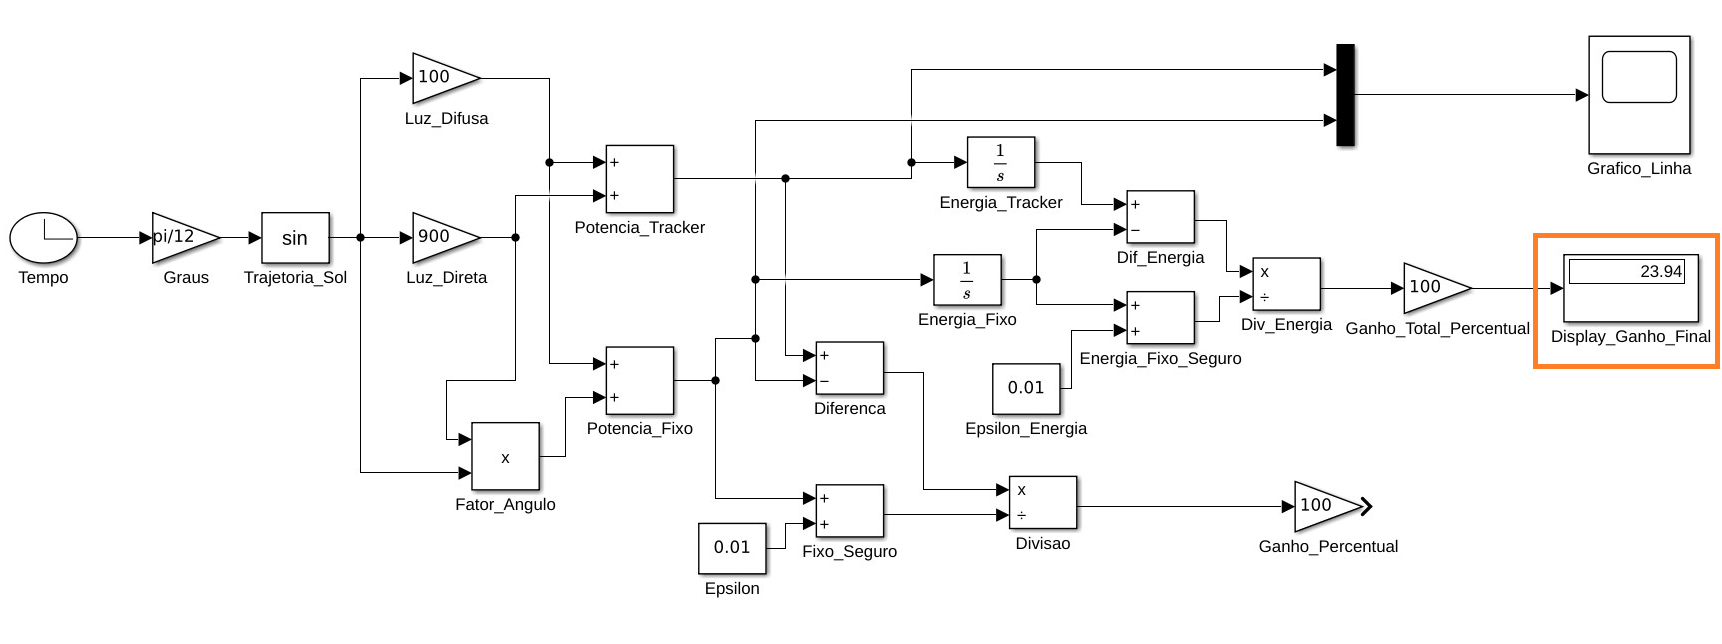
\includegraphics[width=\textwidth]{Figuras/MS.png}
\caption{Modelo computacional desenvolvido no ambiente MATLAB/Simulink.}
\label{fig:simulink_modelo}
\fonte{Autor (2026).}
\end{figure}

O funcionamento do modelo inicia-se com o bloco \textit{Clock}, responsável por fornecer o tempo da simulação. Em seguida, esse sinal é convertido em radianos por um bloco de ganho e aplicado a uma função seno, utilizada para representar de forma simplificada a trajetória aparente do Sol ao longo do dia. A partir desse sinal são geradas as componentes de irradiância empregadas no cálculo da potência produzida pelo sistema automatizado e pelo sistema com painel fixo. Posteriormente, o modelo determina a energia acumulada e o ganho percentual entre as duas configurações, permitindo a comparação dos resultados simulados com os dados obtidos experimentalmente.

De acordo com o Centro de Referência para Energia Solar e Eólica Sérgio de Salvo Brito (CRESESB), a irradiância solar extraterrestre apresenta valor médio próximo de 1361 W/m², conhecido como constante solar \cite{cresesb}. Entretanto, devido aos fenômenos de absorção, reflexão e espalhamento da radiação na atmosfera terrestre, a irradiância disponível na superfície é reduzida. Em condições atmosféricas favoráveis e céu limpo, a irradiância incidente pode atingir aproximadamente 1000 W/m², valor adotado internacionalmente como Condição Padrão de Teste (\textit{Standard Test Conditions} -- STC) para caracterização de módulos fotovoltaicos \cite{solarscope}.

Conforme descrito na Seção~\ref{sec:modelagem_simulacao}, o modelo considera uma irradiância direta máxima de 900 W/m² e uma componente difusa de 100 W/m², totalizando aproximadamente 1000 W/m² nas Condições Padrão de Teste (STC). O período de simulação foi definido em 12 horas, representando o intervalo diário de disponibilidade de radiação solar.

Para o sistema automatizado, considerou-se que o painel permanece continuamente orientado na direção de maior incidência da radiação solar, recebendo integralmente as componentes direta e difusa da irradiância.

No sistema com painel fixo, a componente direta da irradiância foi ponderada por um fator angular, representando as perdas decorrentes do desalinhamento entre o painel e a posição aparente do Sol. Dessa forma, o modelo representa a redução da potência produzida ao longo do dia em função da variação do ângulo de incidência da radiação solar.

As potências instantâneas produzidas pelos dois sistemas foram integradas ao longo do tempo para determinação da energia acumulada durante o período de simulação. Em seguida, foi calculado o ganho percentual do sistema automatizado em relação ao sistema com painel fixo, permitindo comparar diretamente o desempenho energético das duas configurações.

Ao término da simulação, o modelo fornece as curvas de potência dos sistemas automatizado e de painel fixo, além da energia acumulada e do ganho percentual calculado entre as duas configurações. Esses dados foram posteriormente utilizados na comparação com os resultados obtidos experimentalmente.

O código-fonte desenvolvido para a implementação do modelo computacional no MATLAB/Simulink encontra-se disponibilizado no Apêndice~\ref{ap:github}, permitindo a reprodução da simulação apresentada neste trabalho.

\subsection{Validação do Modelo Computacional}
\label{subsec:validacao_modelo}

Após o desenvolvimento do modelo computacional, foi realizada sua validação por meio da comparação entre os resultados obtidos na simulação e os dados experimentais coletados pelo protótipo físico desenvolvido neste trabalho.

Para garantir a comparabilidade entre os resultados, a simulação e os ensaios experimentais foram conduzidos considerando o mesmo período diário de operação e configurações equivalentes para os sistemas fotovoltaicos automatizado e com painel fixo.

A validação consistiu na comparação das curvas das grandezas elétricas obtidas na simulação com aquelas medidas experimentalmente, incluindo tensão elétrica, potência e ganho percentual em relação ao sistema de painel fixo. Além da análise gráfica, foram avaliadas as diferenças entre os valores simulados e experimentais, verificando a capacidade do modelo computacional em representar o comportamento observado no sistema físico.

Os resultados dessa comparação são apresentados e discutidos no Capítulo~\ref{cap5_resultados}, onde é analisado o grau de concordância entre a simulação computacional e o protótipo experimental, permitindo avaliar a representatividade do modelo desenvolvido.

\section{Protocolo Experimental}

Após o desenvolvimento do protótipo e da implementação do modelo computacional, foram realizados ensaios experimentais com o objetivo de comparar o desempenho do sistema fotovoltaico automatizado com o de um sistema de painel fixo. Para garantir a comparabilidade entre os sistemas, ambos foram submetidos às mesmas condições ambientais durante todo o período de coleta de dados, permitindo avaliar a influência do posicionamento automatizado sobre a geração de energia elétrica.

As subseções seguintes descrevem o local de instalação do protótipo, os procedimentos adotados durante os ensaios experimentais e os métodos empregados no tratamento dos dados coletados, os quais foram posteriormente utilizados na comparação com os resultados obtidos pelo modelo computacional.


\subsection{Local de Instalação}

Os ensaios experimentais foram realizados na cidade de Salinas, localizada no norte do estado de Minas Gerais. O protótipo foi instalado em uma área aberta, livre de obstáculos que pudessem provocar sombreamento ao longo do período de coleta de dados, garantindo que os dois sistemas fossem submetidos às mesmas condições de irradiância durante os experimentos.

As coordenadas geográficas aproximadas do local de instalação são:

\begin{itemize}
    \item Latitude: $16,17^\circ$ S;
    \item Longitude: $42,29^\circ$ O.
\end{itemize}

O protótipo foi instalado sobre uma superfície nivelada, proporcionando estabilidade mecânica durante todo o período experimental.

O sistema automatizado realizava o posicionamento do painel fotovoltaico em um único eixo (Leste--Oeste). Diariamente, o painel iniciava sua operação às 06h00 voltado para leste e era movimentado automaticamente em direção ao oeste até as 18h00, acompanhando o deslocamento aparente do Sol.

Para fins de comparação, foi utilizado um segundo painel fotovoltaico com as mesmas especificações, mantido em posição fixa durante todo o período experimental. Esse painel permaneceu instalado horizontalmente ($0^\circ$ em relação ao plano horizontal), sem qualquer ajuste de orientação ou posicionamento, permitindo comparar diretamente o desempenho de um sistema estático com o sistema de posicionamento automatizado desenvolvido neste trabalho.

A configuração horizontal foi adotada para ambos os painéis no instante inicial da montagem, de modo que a principal diferença entre os sistemas estivesse relacionada exclusivamente ao posicionamento automatizado do painel ao longo do dia, eliminando a influência de diferentes ângulos de instalação na comparação dos resultados.

\subsection{Procedimentos Experimentais}

Os ensaios experimentais foram realizados entre os dias 23 e 26 de maio de 2026, período selecionado em função das condições climáticas favoráveis, priorizando dias sem ocorrência de precipitação. Como o protótipo permaneceu instalado em ambiente externo durante toda a campanha experimental, essa condição contribuiu para reduzir interferências decorrentes das condições meteorológicas.

Durante os ensaios, o sistema automatizado e o sistema de painel fixo operaram simultaneamente, permanecendo submetidos às mesmas condições de irradiância ao longo de todo o período de coleta de dados. Essa configuração permitiu comparar diretamente o desempenho das duas configurações, minimizando a influência das variações ambientais sobre os resultados experimentais.

A coleta de dados foi realizada diariamente entre 06h00 e 18h00, intervalo correspondente ao período diário de operação do sistema. No início de cada dia, o painel do sistema automatizado era posicionado na direção leste e, ao longo do período de funcionamento, seu ângulo era ajustado automaticamente de acordo com a estratégia de controle implementada no microcontrolador, finalizando sua movimentação na direção oeste. O painel utilizado como referência permaneceu em posição fixa durante todo o experimento.

As medições de tensão elétrica, corrente elétrica, potência, ângulo de posicionamento, data e horário foram realizadas automaticamente em intervalos de um minuto e registradas em arquivos armazenados no cartão microSD. Esses registros constituíram a base de dados utilizada para a comparação entre o sistema automatizado, o sistema de painel fixo e os resultados obtidos pelo modelo computacional desenvolvido no MATLAB/Simulink.

Ao término de cada dia de coleta, os arquivos gerados foram transferidos para um computador, onde passaram pelas etapas de organização e verificação dos dados. Posteriormente, essas informações foram utilizadas na elaboração dos gráficos, tabelas e análises apresentados no Capítulo de Resultados. Os registros completos obtidos durante os ensaios experimentais encontram-se apresentados no Apêndice~\ref{ap:apendiceC}.

\subsection{Tratamento dos Dados}

Os dados registrados pelos sistemas foram exportados para planilhas eletrônicas, onde passaram pelas etapas de organização, conferência e processamento para obtenção dos resultados apresentados neste trabalho.

Inicialmente, os registros foram verificados para identificar possíveis inconsistências decorrentes do processo de aquisição dos dados. Em seguida, foram calculadas as variáveis de interesse, incluindo a potência instantânea, a energia acumulada ao longo do período de operação e o ganho percentual do sistema automatizado em relação ao sistema com painel fixo.

A potência elétrica instantânea foi calculada a partir das medições de tensão e corrente, conforme a Equação~\ref{eq:potencia}.

O ganho percentual de energia do sistema automatizado em relação ao sistema de painel fixo foi determinado pela Equação~\ref{eq:ganho}.

Os resultados obtidos experimentalmente foram organizados em tabelas e gráficos, possibilitando a comparação entre os dois sistemas. Posteriormente, esses resultados também foram comparados aos valores obtidos pelo modelo computacional desenvolvido no MATLAB/Simulink, por meio da análise dos perfis de potência, da energia acumulada e do ganho percentual de energia. Essa etapa permitiu avaliar a capacidade do modelo computacional em representar o comportamento observado no protótipo físico.
